\documentclass[../main.tex]{subfiles}
\graphicspath{{\subfix{..}}}

\begin{document}
\chapter{Machine learning and Artificial Neural Network}
\label{sec:ml}

\epigraph{``I have the shape of a human being and organs equivalent to those of a human being. My organs, in fact, are identical to some of those in a prosthetized human being. I have contributed artistically, literally, and scientifically to human culture as much as any human being now alive. What more can one ask?''}{Isaac Asimov, The Complete Robot }

Machine Learning (ML) and more specifically Neural Network (NN) are families of data-driven algorithm. They are used to model complex distributions from a finite dataset to extract a generalist behavior. They learn, adapt their intrinsic parameters, interactively by computing its performance or \textit{loss} on those dataset. They take advantage of simple microscopic operation such as \textit{if condition} or non-continuous but differentiable function like \textit{ReLU}. Through optimizers and the combination of a lot of those microscopic operations, they can obtain complex and precise behaviours.

They are now widely used in a wide variety of domain including natural language processing, computer vision, speech recognition and, the subject of this thesis, scientific studies.

We found them in particle physics, either as the main algorithm or as secondary algorithm, for event reconstruction, event classification, waveform reconstruction, etc..., domains where the underlying physic and detector process is complex and highly dimensional. Physicists have traditionally been forced to use simplifications or assumptions to ease the developmment of algorithms or equations (a good example is the algorithm presented in section \ref{sec:juno:reco}) where machine learning could refine and take into account those effects, provided that they have enough data and computing power.

This chapter present an overview of the different kind of machine learning methods and neural networks that will be discussed in this thesis.
\section{Boosted Decision Tree (BDT)}
\label{sec:ml:bdt}

One of the most classic machine learning algorithm used in particle physics is Boosted Decision Tree (BDT) \cite{breiman_classification_2017} (or more recently Gradient Boosting Machine \cite{friedman_greedy_2001}). The principle of a BDT is fairly simple : based on a set of observables, a serie of decisions, represented as node in a tree, are taken by the algorithm. Each decision point, or node, takes its decision based on a set of trainable parameters leading to a subtree of decision. The process is repeated until it reach the final node, yielding the prediction. A simplistic example is given in figure \ref{fig:ml:bdt}.

\begin{figure}
  \centering
  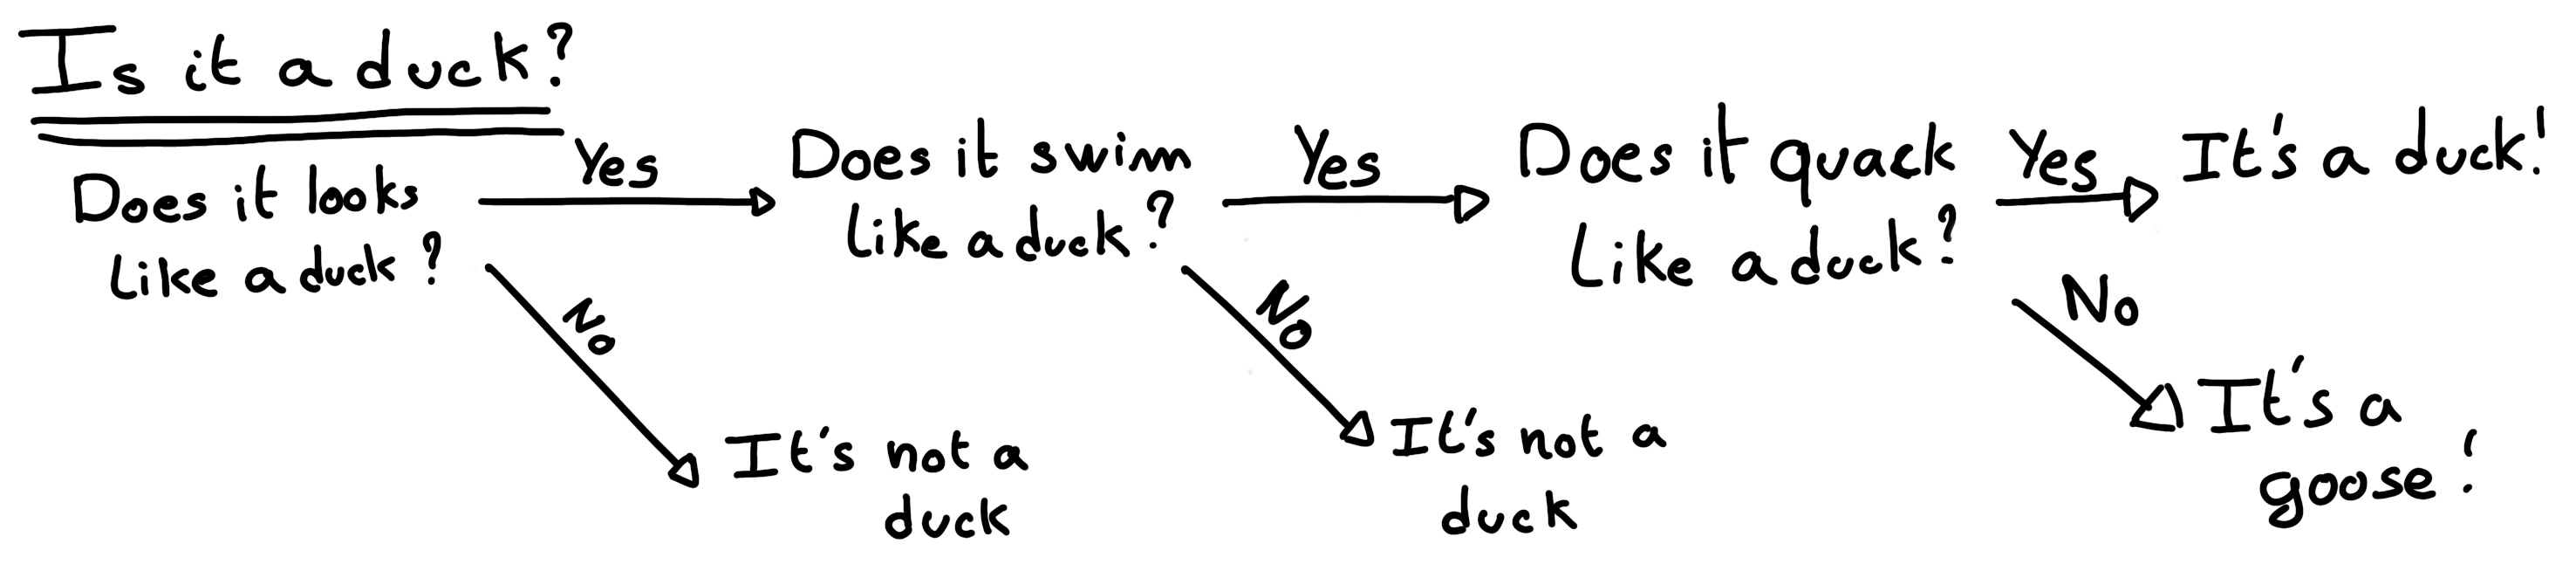
\includegraphics[width=\linewidth]{images/ml/Bdt.jpg}
  \caption{Example of a BDT that determine if the given object is a duck}
  \label{fig:ml:bdt}
\end{figure}

The training procedure follow a simple score reward procedure. During the training phase the prediction of the BDT is compared to a known truth about the data. The score is then used to backpropagate corrections to the parameters of the tree. Modern BDT use gradient boosting where the gradient of the loss is calculated for each of the BDT parameters. Following the gradient descent, we can reach the, hopefully, global minima of the loss for our set of parameters.

\section{Artificial Neural Network (NN)}
\label{sec:ml:nn}

One other big family of machine learning algorithm is the artificial Neural Networks (NN). The idea of developing automates which component mimic, in a simplistic way, the behavior of biological neurons emerge in 1959 with the paper ``\textit{What the Frog's Eye Tells the Frog's Brain}'' \cite{lettvin_what_1959}. They develop an automate where each component possess an \textit{activation function}. Each one of those component then transmit its information to the other following a certain efficiency or \textit{weight}.
Those works influenced scientist and notably Frank Rosenblatt who published in 1958 what is considered the first neural network model the Perceptron \cite{rosenblatt_perceptron_1958}.


Modern neural network still nowadays use the neuron metaphor to represent neural network, but approach them as a graph where the nodes are neurons possessing an activation function and edges holding the weights, or \textit{parameters} in modern literature, between those nodes. Most of the modern neural network work with the principle of neurons layers. Each neurons belong to a layer and takes input from the preceding layer and forward it result to next layer. For example the most basic set layer is the fully connected layer where each of its neurons is connected to every other neurons of the precessing layer. All the neurons posses the same activation function $F$. The connection between two the two layers is expressed as a tensor $T^{i}_{j}$ where $i$ is the index of the precedent layer and $j$ the index of the current layer. The propagation from the layer $I$ to $J$ is then described as
\begin{equation}
  \label{eq:ml:fully-connected}
  J_{j} = F_J(T_{j}^{i} I_{i} + B_j)
\end{equation}
where the learning parameters are the tensor $T_j^i$ and the bias tensor $B_j$. This is the fundamental component of the Fully Connected Deep NN (FCDNN) family presented in section \ref{sec:ml:fcdnn}. Most of the modern neural networks use gradient descent to optimize their parameters, i.e. the gradient of the parameter $\theta$ in respect of the loss function $\mathcal{L}$ is subtracted to it
\begin{equation}
  \theta_{i+1} = \theta_i - \frac{\partial \mathcal{L}}{\partial \theta}
\end{equation}
$i$ being the training iteration index. This needs the expression of $\mathcal{L}$ dependent of $\theta$ to be differentiable, thus the layer and their activation function also need to be differentiable. This simple gradient descent, designated as Stochastic Gradient Descent (SGD), can be completed with first and second order momentum like with the Adam optimizer \cite{kingma_adam_2017} (more details in section \ref{sec:ml:train}).

This description of neural networks as layer introduced the principle of \textit{depth} and \textit{width}, the number of layers in the NN and the number of neurons in each layer respectively. Those quantities that not directly used for the computation of the results but describe the NN or its training are designated as \textit{hyperparameters}.

The loss $\mathcal{L}$ described above is a score representing how well the NN is doing. As seen above, it needs to be differentiable with respect to the parameter of the NN. Depending if we try to minimize or maximize it, it need to posses a minima or a maxima. For example when doing \textit{regression}, i.e. produce a scalar result, a common loss is the Mean Square Error (MSE). Let $i$ be our dataset, $y_i$ be the target scalar, $x_i$ the input data and $f(x_i, \mathbb{\theta})$ the result of the network. The network here is modelled by $f$, and its parameter by the set $\mathbb{\theta}$
\begin{equation}
  \mathcal{L} \coloneq MSE = \frac{1}{N} \sum_i^N (y_i - f(x_i))^2
\end{equation}
Another common loss function is the Mean Absolute Error (MAE)
\begin{equation}
  \mathcal{L} \coloneq MAE = \frac{1}{N} \sum_i^N |y_i - f(x_i)|
\end{equation}


\subsection{Fully Connected Deep Neural Network (FCDNN)}
\label{sec:ml:fcdnn}

Fully Connected Deep Neural Network (FCDNN) architecture is the natural evolution of the Perceptron. The input data is represented as a first order tensor $I_j$ and then fed forward to multiple fully connected layers (Eq \ref{eq:ml:fully-connected}) as presented in the figure \ref{fig:ml:fcdnn}. Most of the time, the classic ReLU function
\begin{equation}
  \label{sec:ml:relu}
  \mathrm{ReLU}(x) = \begin{cases}
    x & \mathrm{if} ~ x \geq 0 \\
    0 & \mathrm{otherwise}
  \end{cases}
\end{equation}
is used as activation function. Prelu and Sigmoid are also popular choices:


\begin{minipage}{0.5\linewidth}
  \begin{equation}
    \label{sec:ml:sigmoid}
    \mathrm{Sigmoid}(x) = \frac{1}{1+ e^{-x}}
  \end{equation}
\end{minipage}
\begin{minipage}{0.5\linewidth}
  \begin{equation}
    \label{sec:ml:prelu}
    \mathrm{PReLU}(x) = \begin{cases}
      x & \mathrm{if} ~ x \geq 0 \\
      \alpha x & \mathrm{otherwise}
    \end{cases}
  \end{equation}
\end{minipage}


The reasoning behind ReLU and PReLU is that with enough of them, you can mimic any continuous function as illustrated in figure \ref{fig:ml:relu-mimic}. Sigmoid is more used in case of classification, its behavior going hand in hand with the Cross Entropy loss function used in classification problems.

\begin{figure}[ht]
  \begin{subfigure}[t]{0.48\textwidth}
    \centering
    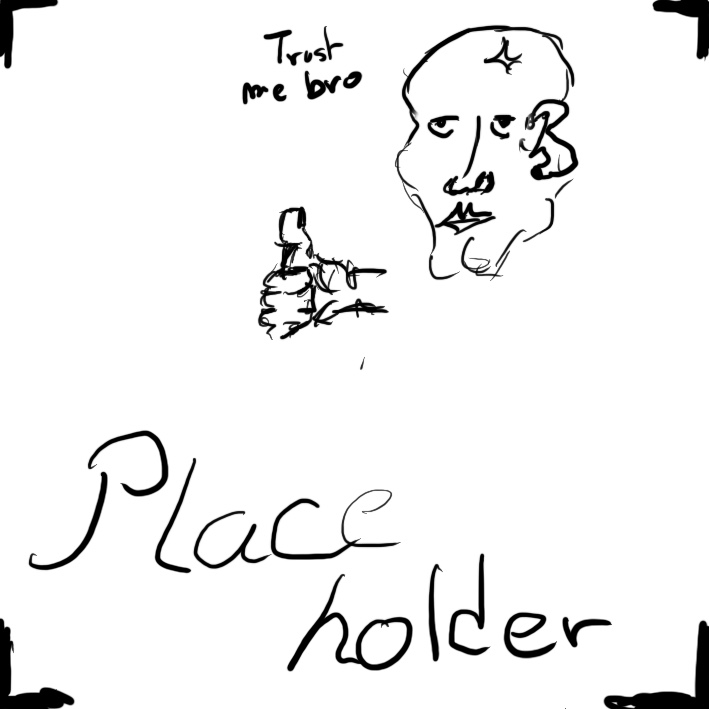
\includegraphics[height=6cm]{images/placeholder.jpg}
    \caption{Schema of a FCDNN}
    \label{fig:ml:fcdnn}
  \end{subfigure}
  \hfill
  \begin{subfigure}[t]{0.48\textwidth}
    \centering
    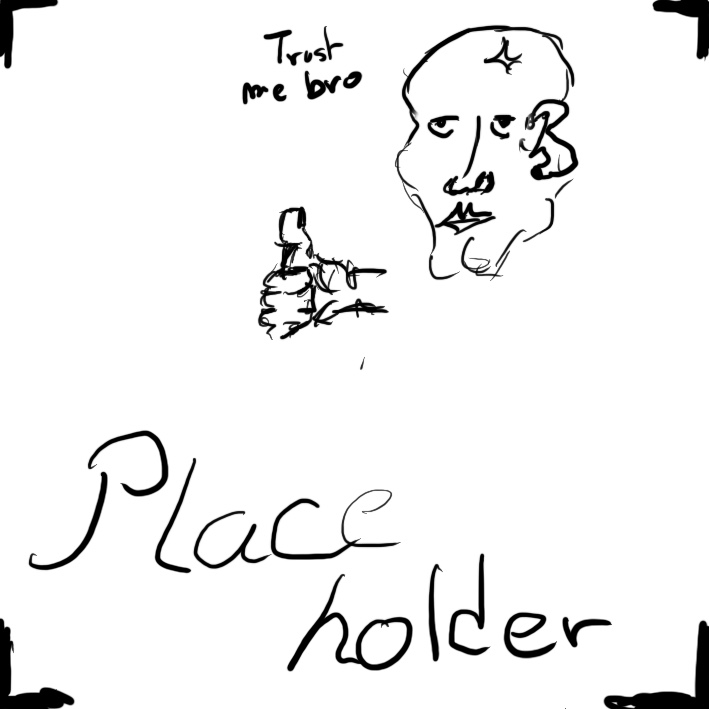
\includegraphics[height=6cm]{images/placeholder.jpg}
    \caption{Illustration of a composition of ReLU matching a function}
    \label{fig:ml:relu-mimic}
  \end{subfigure}
  \caption{}
\end{figure}

Due to its simplicity, FCDNN are also used as basic pieces for more complex architectures such as the CNN and GNN that will be presented in the next section.

\subsection{Convolutional Neural Network (CNN)}
\label{sec:ml:cnn}

Convolutional Neural Networks are a family of neural networks that use discrete convolution filters, as illustrated in an example in figure \ref{fig:ml:conv_filter}, to process the input data, often images. They have the advantage to be translation invariant by construction, this mean that they are capable of detecting oriented features independently of their location on the image. The learning parameters are located in the filters, the network thus learn the optimal filters to extract the desired features. 2D CNN, where the filters are second order tensors that span over third order tensors, are commonly used in image recognition \cite{russakovsky_imagenet_2015} for classification or regression problematics.

The convolution layers are commonly chained \cite{simonyan_very_2015}, reducing the input dimension while increasing the number of filters. The idea behind is that the first layers will process local informations and the latest layers will process more global informations. To try to preserve the amount of information, we tend to double the numbers of filters for each division of the input data.
The results of the convolution filters is commonly then flattened and feed to a smaller FCDNN which will process the filters results to yield the desired output.

\begin{figure}[ht]
  \centering
  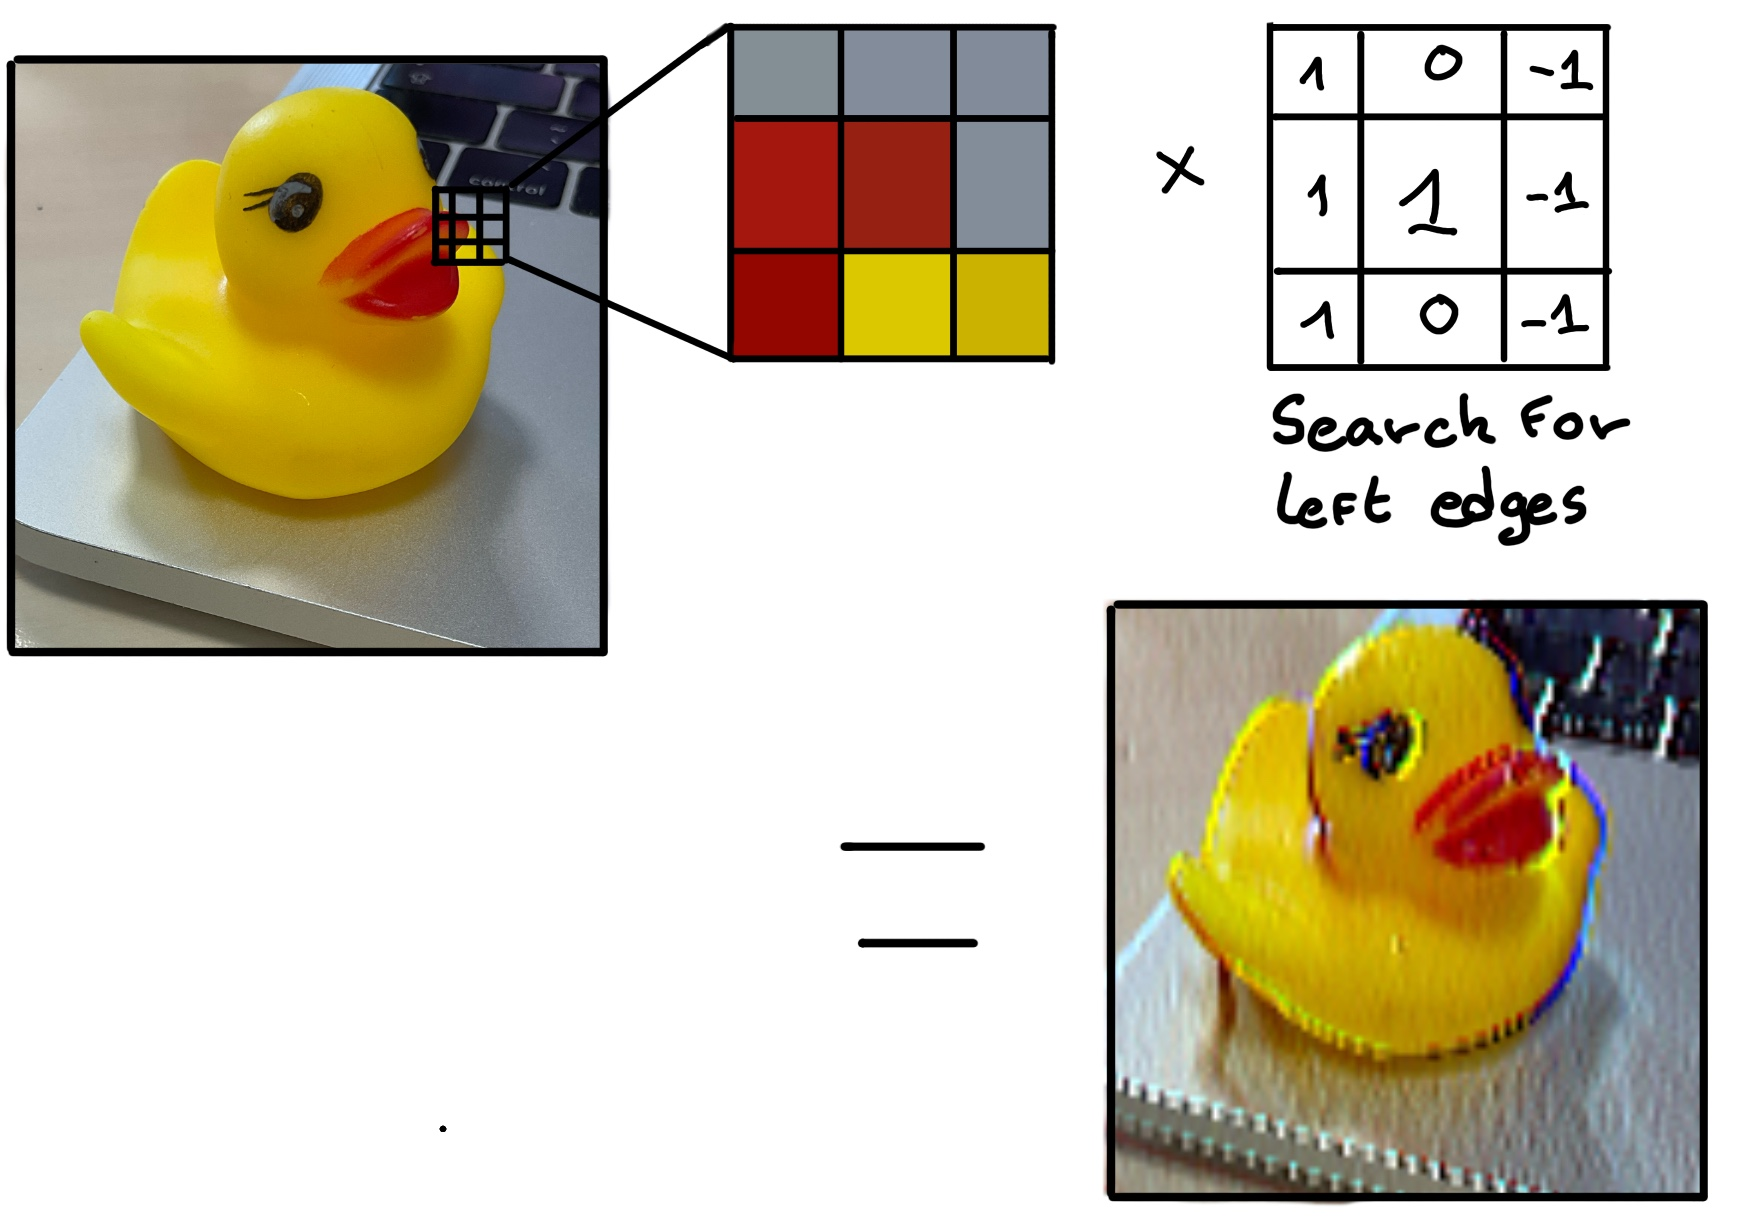
\includegraphics[height=6cm]{images/ml/convolution_exammple.jpg}
  \caption{Illustration of the effect of a convolution filter. Here we apply a filter with the aim do detect left edges. We see in the resulting image that the left edges of the duck are bright yellow where the right edges are dark blue indicating the contour of the object. The convolution was calculated using \cite{allen_generic-github-userimage-convolution-playground_2024}.}
  \label{fig:ml:conv_filter}
\end{figure}

As an example, let's take the Pytorch \cite{ansel_pytorch_2024} example for the MNIST \cite{lecun_gradient-based_1998}, a dataset of black and white images of handwritten digits. Those images are $28 \times 28$ pixels with only one channel corresponding to the grey level of the pixel. Example of images from this dataset are presented in figure \ref{fig:ml:mnist}

A schema of the CNN used in the Pytorch example is presented in figure \ref{fig:ml:cnn_mnist}. Using this schema as a reference, the trained network is made of:
\begin{enumerate}
  \item A convolutional layer of $(3 \times 3)$ filters yielding 32 channels. A bias parameter is applied to each channel for a total of $(32 \cdot (3\times3) + 32) = 320$ parameters. The resulting image is $(26\times26 \times 32)$ (26 per 26 pixels with 32 channels). The ReLU activation function is applied to each pixel.
  \item A second convolutional layer of $(3 \times 3)$ filters yielding 64 channels. This channel also posses a bias parameter for a total of $(64 \cdot (3\times3) + 64) = 640$ parameters. Resulting image is $(24\times24\times64)$. Also with with a ReLU activation function.
  \item Then comes a $(2\times2)$ max pool layer with a stride of 1 meaning that for each channel the max value of pixels in a $(2\times2)$ block is condensed in a single resulting pixel. The resulting image is $(12 \times 12 \times 64)$.
  \item This image goes through a dropout layer which will set the pixel to 0 with a probability of 0.25. This help prevent overtraining of the neural network (see section \ref{sec:ml:pitfall} for more details).
  \item The data is the flattened i.e. condensed into a vector of $(12 \times 12 \times 64) = 9216$ values.
  \item Then comes a fully connected linear layer (Eq. \ref{eq:ml:fully-connected}) with a ReLU activation that output 128 feature. It needs $(9216 \cdot 128)+ 128 = 1'179'776$ parameters.
  \item This 128 item vector goes through another dropout layer with a probability of $0.5$
  \item The vector is then transformed through a linear layer with ReLU activation. It output 10 values, one for each digit class (0, 1, 2, ..., 9). It need $(128 \cdot 10) + 128 = 1408$ parameters.
  \item Finally the 10 values are normalized using a log softmax function $\mathrm{LogSoftmax}(x_i) = \log \bigg(\frac{\exp(x_i)}{\sum_j \exp(x_j)}\bigg)$ to give the probability of the input image to be a certain digit.
\end{enumerate}

\begin{figure}[ht]
  \centering
  \begin{subfigure}[t]{0.48\linewidth}
    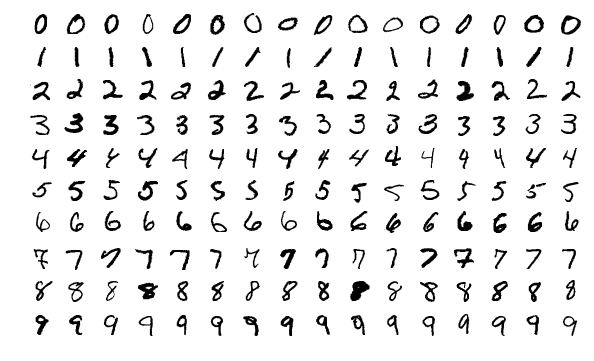
\includegraphics[width=\linewidth]{images/ml/MnistExamples.png}
    \caption{Example of images in the MNIST dataset}
    \label{fig:ml:mnist}
  \end{subfigure}
  \hfill
  \begin{subfigure}[t]{0.48\linewidth}
    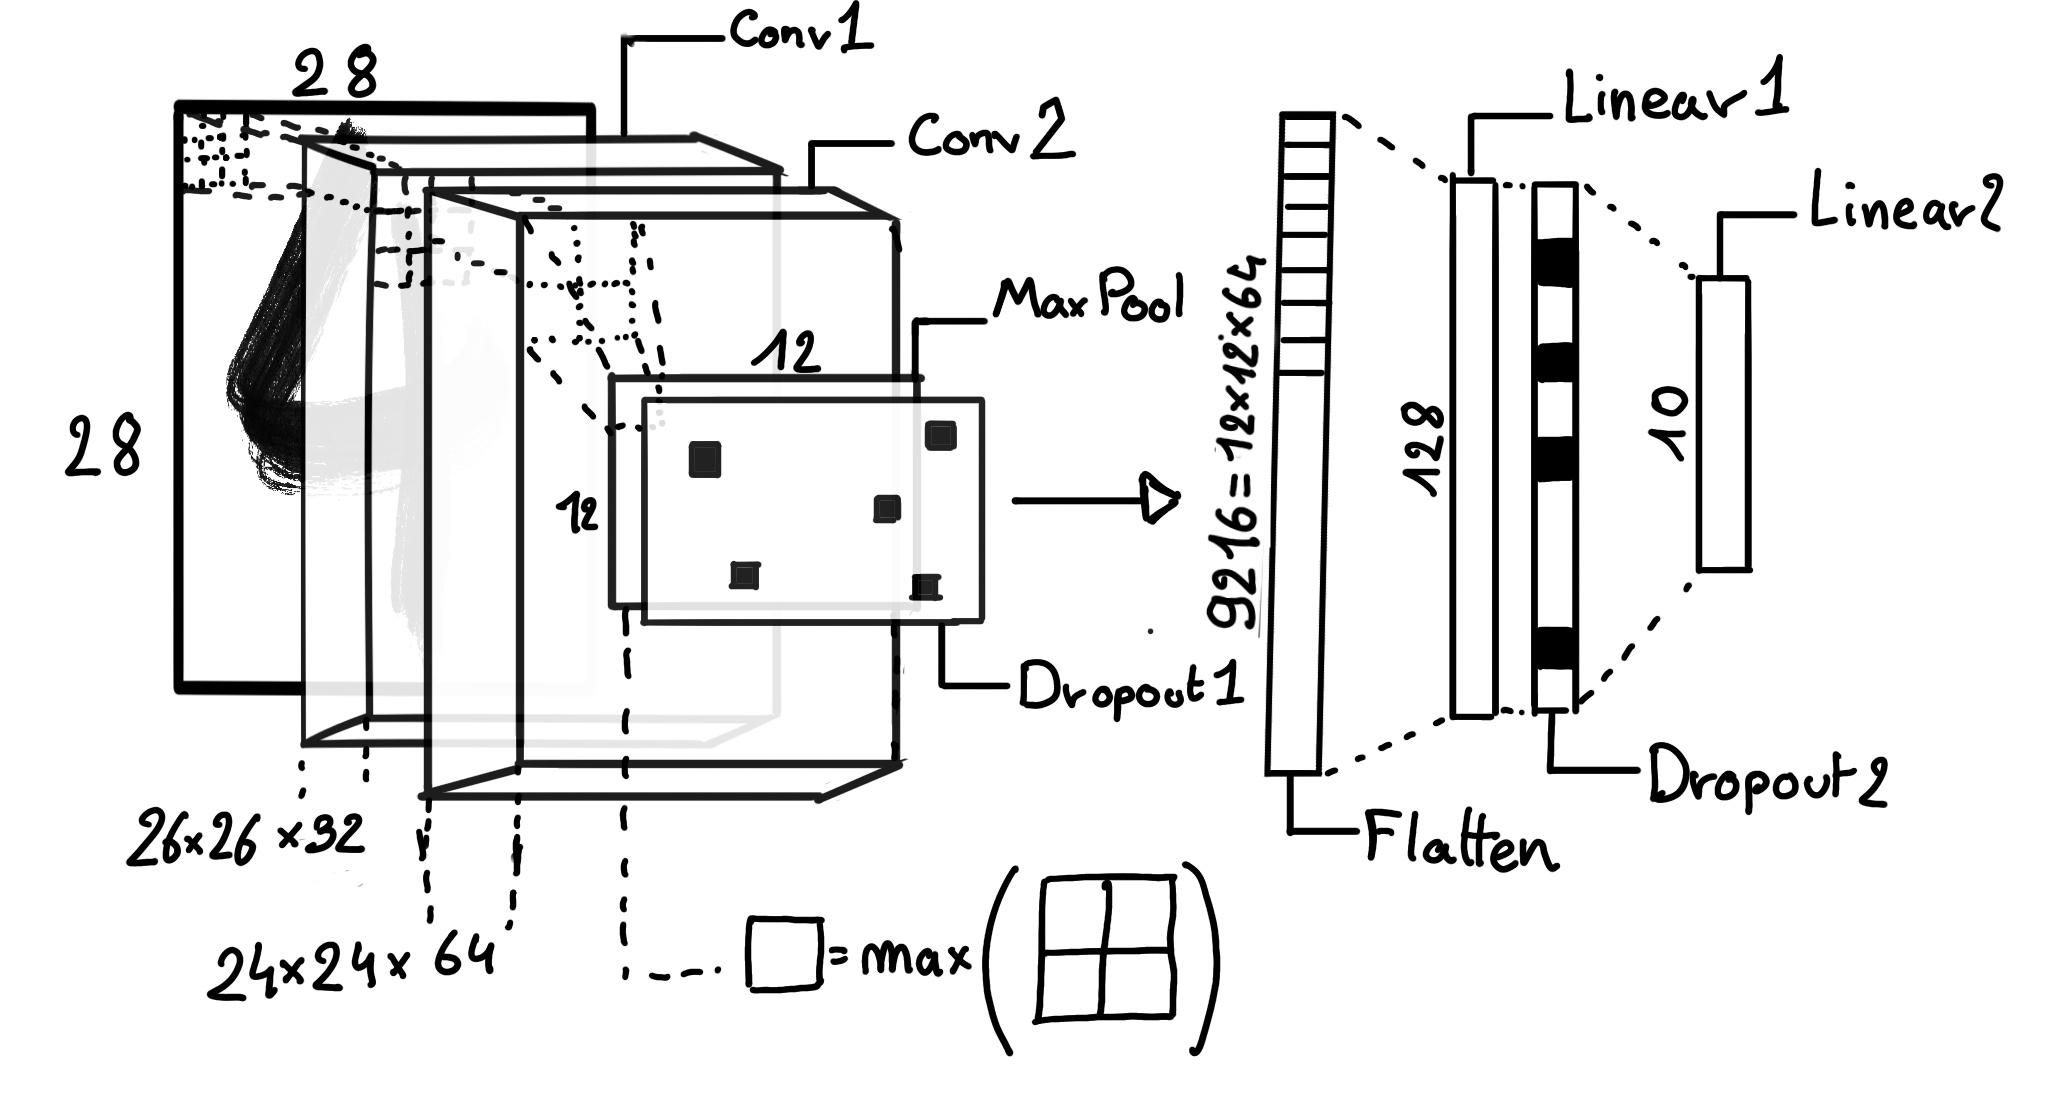
\includegraphics[width=\linewidth]{images/ml/mnist_cnn.jpg}
    \caption{Schema of the CNN used in Pytorch example to process the MNIST dataset}
    \label{fig:ml:cnn_mnist}
  \end{subfigure}
  \caption{}
\end{figure}

The final network needs 1'182'144 parameters or, if we consider each parameters to be a double precision floating point, 9.45 MB of data. To gives a order of magnitude, such neural network is considered ``simple'', train in a matter of minutes on T4 GPU \cite{noauthor_nvidia_nodate} (14 epochs) and reach an accuracy in its prediction of 99\%.


\subsection{Graph Neural Network (GNN)}

Graph neural network is a family of neural network where the data is represented as a graph $G(\mathcal{N},\mathcal{E})$ composed of vertex or node $n \in \mathcal{N}$ and edges $e \in \mathcal{E}$. The edges are associated to two nodes $(u, v) \in \mathcal{N}^2$, ``connecting'' them. The node and the edges can hold features, commonly represented as vector $n \in \mathbb{R}^{k_{n}}$, $e \in \mathbb{R}^{k_{e}}$. We can thus define a graph using two tensors $A^{ij}_{\epsilon}$ the adjacency tensors that hold the features $\epsilon$ of the edge connecting the node $i$ and $j$ and the tensor $N^{i}_{\nu}$ that hold the features $\nu$ of a node $i$.

To efficiently manipulate such object we need to structurally encode their property in the neural network architecture: each node is equivalent (as opposite to ordered data in a vector), each node has a set of neighbours, ... One of this method is the message passing algorithm presented historically in ``Neural Message Passing for Quantum Chemistry'' \cite{gilmer_neural_2017}. In this algorithm, with each layer of message passing a new set of features is computed for each node following
\begin{equation}
  n_i^{k+1} = \phi_u (n_i^k, \Box_j \phi_m(n_i^k, n_j^k, e^k_{ij})); ~ n_j \in \mathcal{N}'_i
\end{equation}
where $\phi_u$ is a differentiable update function, $\Box_j$ is a differentiable aggregation function and $\phi_m$ is a differentiable message function. $\mathcal{N}'_i = \{n_j \in \mathcal{N} | (n_i, n_j) \in \mathcal{E}\}$ is the set of neighbours of $n_i$, i.e. the nodes $n_j$ from which it exist an edge $e_{i,j} \rightarrow (n_i, n_j)$. $k$ is the layer on which the message passing algorithm is applied. $\Box$ need also a few other property if we want to keep the graph property, most notably the permutational invariance of its parameters (example: mean, std, sum, ...).

The edges features can also be updated, either by directly taking the results of $\phi_m$ or by using another message function $\phi_e$.


Message passing is a very generic way of describing the process of GNN and it can be specialized for convolutional filtering \cite{defferrard_convolutional_2017}, diffusion \cite{li_diffusion_2018} and many other specific operation. GNN are used in a wide variety of application such as regression problematics, node classification, edge classification, node and edge prediction, ...


It is a very versatile but complex tool.

\subsection{Adversarial Neural Network (ANN)}

The adversarial machine learning, Adversarial Neural Networks (ANN) in the case of neural network, is a family of unsupervised machine learning algorithms where the learning algorithm (generator) is competing against another algorithm (discriminator). Taking the example of Generative Adversarial Networks, concept initially developed by Goodfellow et al. \cite{goodfellow_generative_2014}, the discriminator goal is to discriminate between data coming from a reference dataset and data produced by the generator.
The generator goal, on the other hand, is to produce data that the discriminator would not be able to differentiate from data from the reference dataset. The expression of duality between the two models is represented in the loss where, at least a part of it, is driven by the results of the discriminator.

\subsection{Training procedure}
\label{sec:ml:train}

A neural network without the adequate training is like an empty shell. If the parameters are not optimized they are, most of the time, initialized to random number and so the output will just be random. The training is a key step in the production of a solid and reliable NN. This section aim to give an overview of the different concept and tools used in the training of our neural networks.

\subsubsection{Training lifecycle}

The training of NN does not follow strict rules, you could imagine totally different lifecycle but I will describe here the one used in this thesis, the most common one.

The training is split into \textit{epochs} during which the NN will train on a set of subsamples called \textit{batch}. The size of those batch is called \textit{batch size}, a.k.a. the number of data it contains (how many images, how many events,...). Each process of a batch is called a \textit{step}. At the end of each epochs, the neural network is evaluated over a validation dataset. This validation dataset is not used for training (no gradient of the loss is computed) and is used as reference for the network performance and monitor overtraining (see section \ref{sec:ml:pitfall}). Most of the time, the parameters are updated at each step using the mean loss over the batch and the optimizer hyperparameters are updated at each epochs.

\subsubsection{The optimizer}

As briefly introduced section \ref{sec:ml:nn}, the parameters of the neural network are optimized using the gradient descent method. We calculate the gradient of the mean loss over the batch with respect of each parameters and we update the parameters in accord to minimize the loss. The  gradient is computed backward from the loss up to the first layer parameters using the chain rule:
\begin{equation}
  \label{eq:ml:backward}
  \frac{\partial \mathcal{L}}{\partial \theta_1} = \frac{\partial \theta_2}{\partial \theta_1} \frac{\partial \mathcal{L}}{\partial \theta_2} = \frac{\partial \theta_2}{\partial \theta_1} \frac{\partial \theta_3}{\partial \theta_2} \frac{\partial \mathcal{L}}{\partial \theta_3} = \frac{\partial \theta_2}{\partial \theta_1} \prod_{i=2}^{N-1} \frac{\partial \theta_{i+1}}{\partial \theta_i} \frac{\partial \mathcal{L}}{\partial \theta_N}
\end{equation}
where $\theta$ is a parameter, $i$ is the layer index. We see here that the gradient of the first layer is dependent of the gradient of all the following layers. We thus need to compute the gradient closest to loss first before computing the gradient of the earlier layers. This is called the \textit{backward propagation}.

This update of the parameters is done following an optimizer policy. Those optimizers depends on hyperparameters. The ones used in this thesis are:

\begin{enumerate}
  \item SGD (Stochastic Gradient Descent). This is the simplest optimizer, it depend on only one hyperparameter, the learning rate $\lambda$ (LR) and update the parameters $\theta$ following \begin{equation}
      \theta_{t+1} = \theta_t - \lambda \frac{\partial \mathcal{L}}{\partial \theta}\bigg|_{\theta_t}
    \end{equation}
    where $t$ is the step index. It is a powerful optimizer but is very sensible to local minima of the loss in the parameters phase space as illustrated in figure \ref{fig:ml:sgd}.

  \item Adam \cite{kingma_adam_2017}. The concept is, in short, to have and SGD but with momentum. Adam possess two momentum $m(\beta_1)$ and $v(\beta_2)$ which are respectively proportional to $\frac{\partial \mathcal{L}}{\partial \theta}$ and $(\frac{\partial \mathcal{L}}{\partial \theta})^2$. $\beta_1$ and $\beta_2$ are hyperparameters that dictate the moment update at each optimization step. The parameters are then upgraded following \begin{align}
      m_{t+1} &= \beta_1 m_t + (1 - \beta_1) \frac{\partial \mathcal{L}}{\partial \theta} \\
      v_{t+1} &= \beta_2 v_t + (1 - \beta_2) \bigg(\frac{\partial \mathcal{L}}{\partial \theta}\bigg)^2 \\
      \theta_{t+1} &= \theta{i} - \lambda \frac{m_{t+1}}{\sqrt{v_{t+1}} + \epsilon}
    \end{align}
    where $\epsilon$ is a small number to prevent divergence when $v$ is close to 0. These momentums allow to overcome small local minima in the parameters phase space as illustrated in figure \ref{fig:ml:sgd}.
\end{enumerate}

\begin{figure}
  \centering
  \begin{subfigure}[t]{0.48\linewidth}
    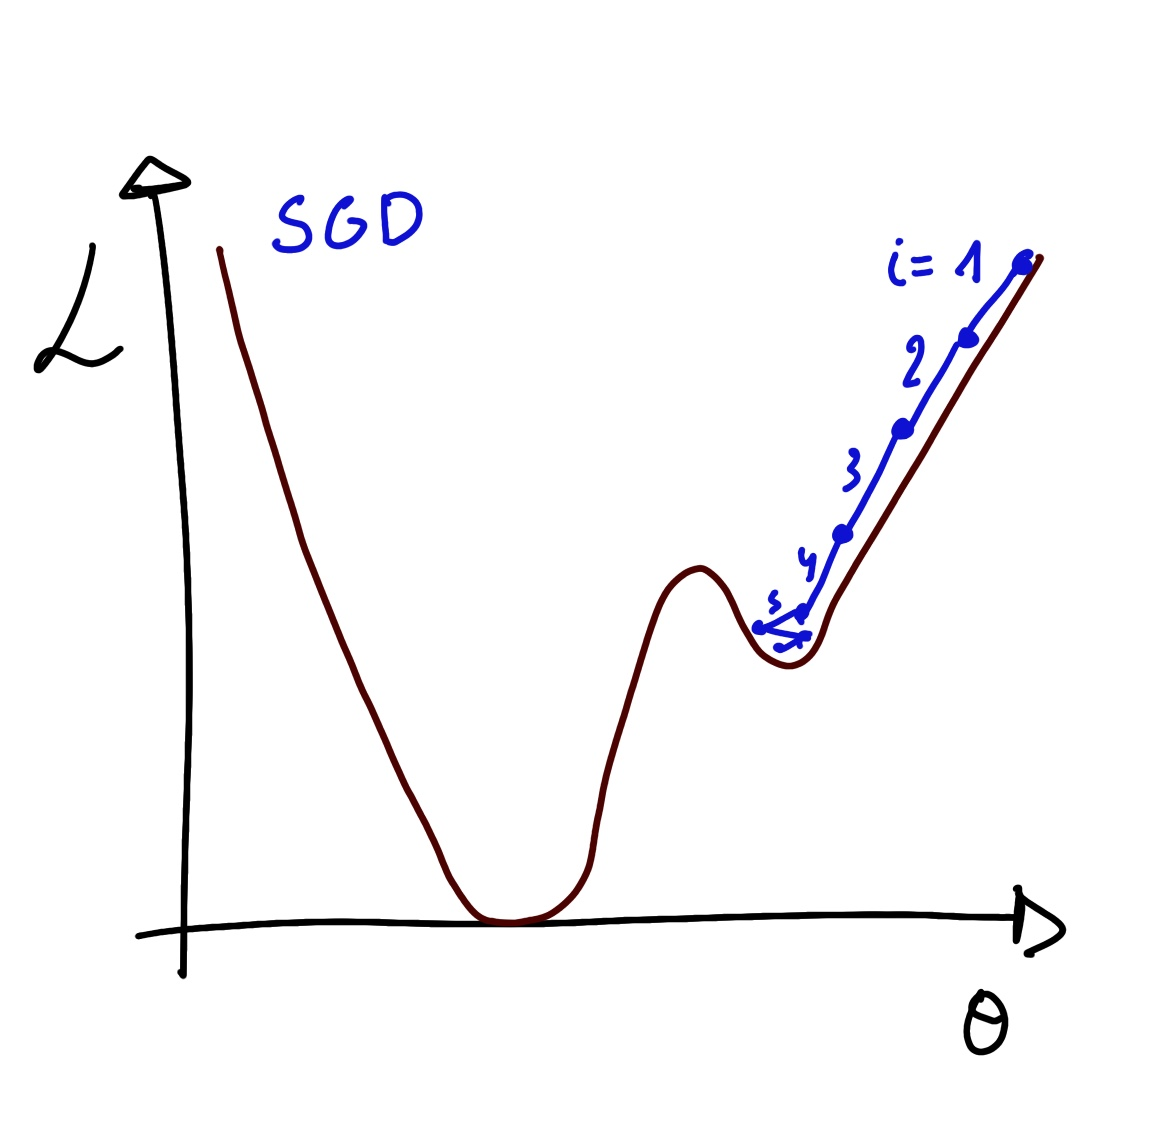
\includegraphics[height=6cm]{images/ml/sgd.jpg}
    \caption{Illustration of SGD falling into a local minima}
    \label{fig:ml:sgd}
  \end{subfigure}
  \hfill
  \begin{subfigure}[t]{0.48\linewidth}
    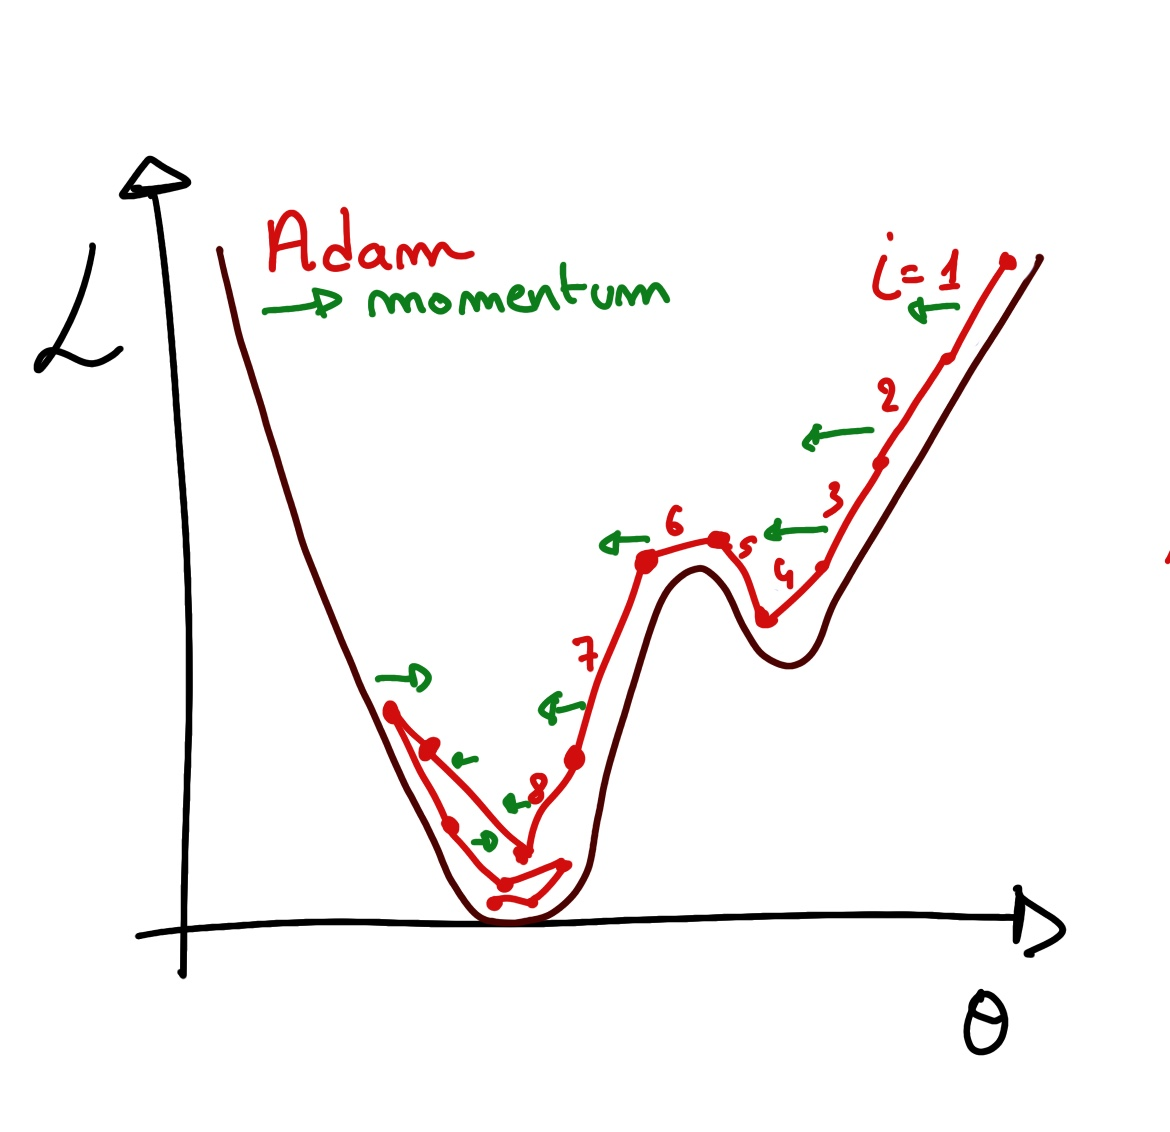
\includegraphics[height=6cm]{images/ml/Adam.jpg}
    \caption{Illustration of the Adam momentum allowing it to overcome local minima}
    \label{fig:ml:adam}
  \end{subfigure}
  \caption{}
\end{figure}

The LR is a crucial parameter in the training of NN, as illustrated in figure \ref{fig:ml:optims}. To prevent possible issues, we setup scheduler policies.

\begin{figure}
  \centering
  \begin{subfigure}[t]{0.48\linewidth}
    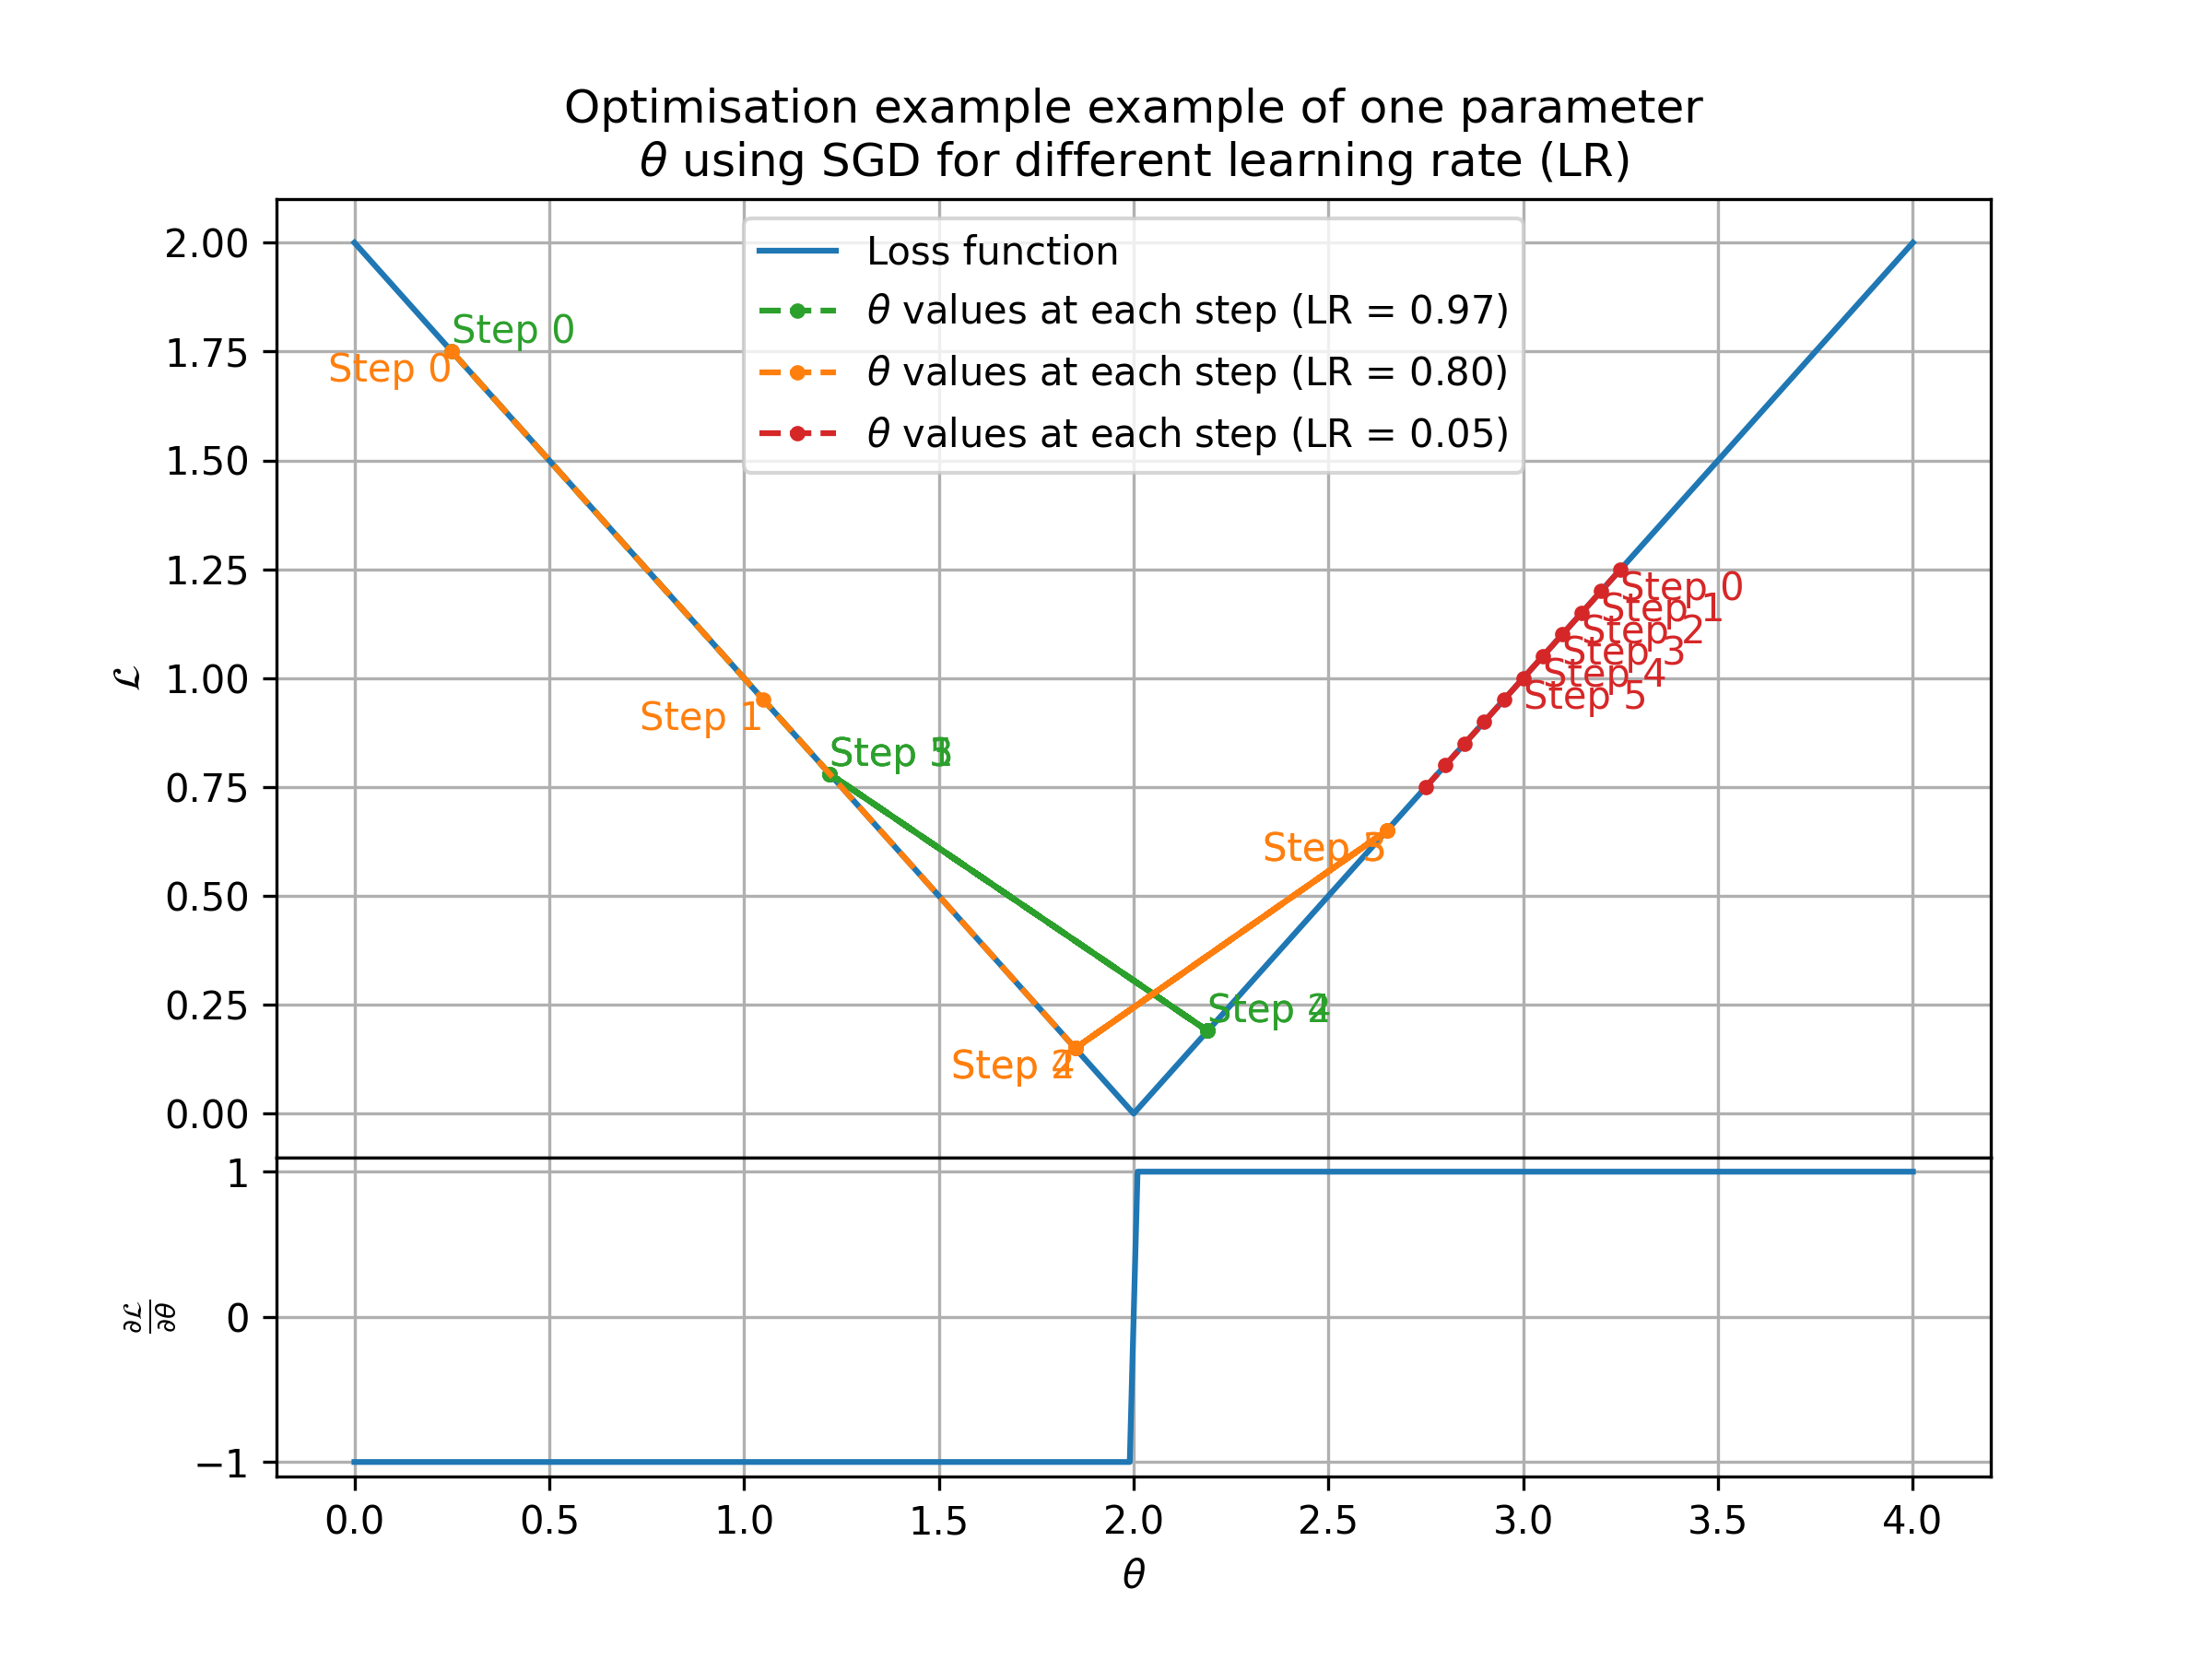
\includegraphics[height=6cm]{scripts/plots/MAE_illustration.png}
    \caption{Illustration of the SGD optimizer on one parameter $\theta$ on the MAE Loss. We see here that it has trouble reaching the minima due to the gradient being constant.}
    \label{fig:ml:optims:mae}
  \end{subfigure}
  \hfill
  \begin{subfigure}[t]{0.48\linewidth}
    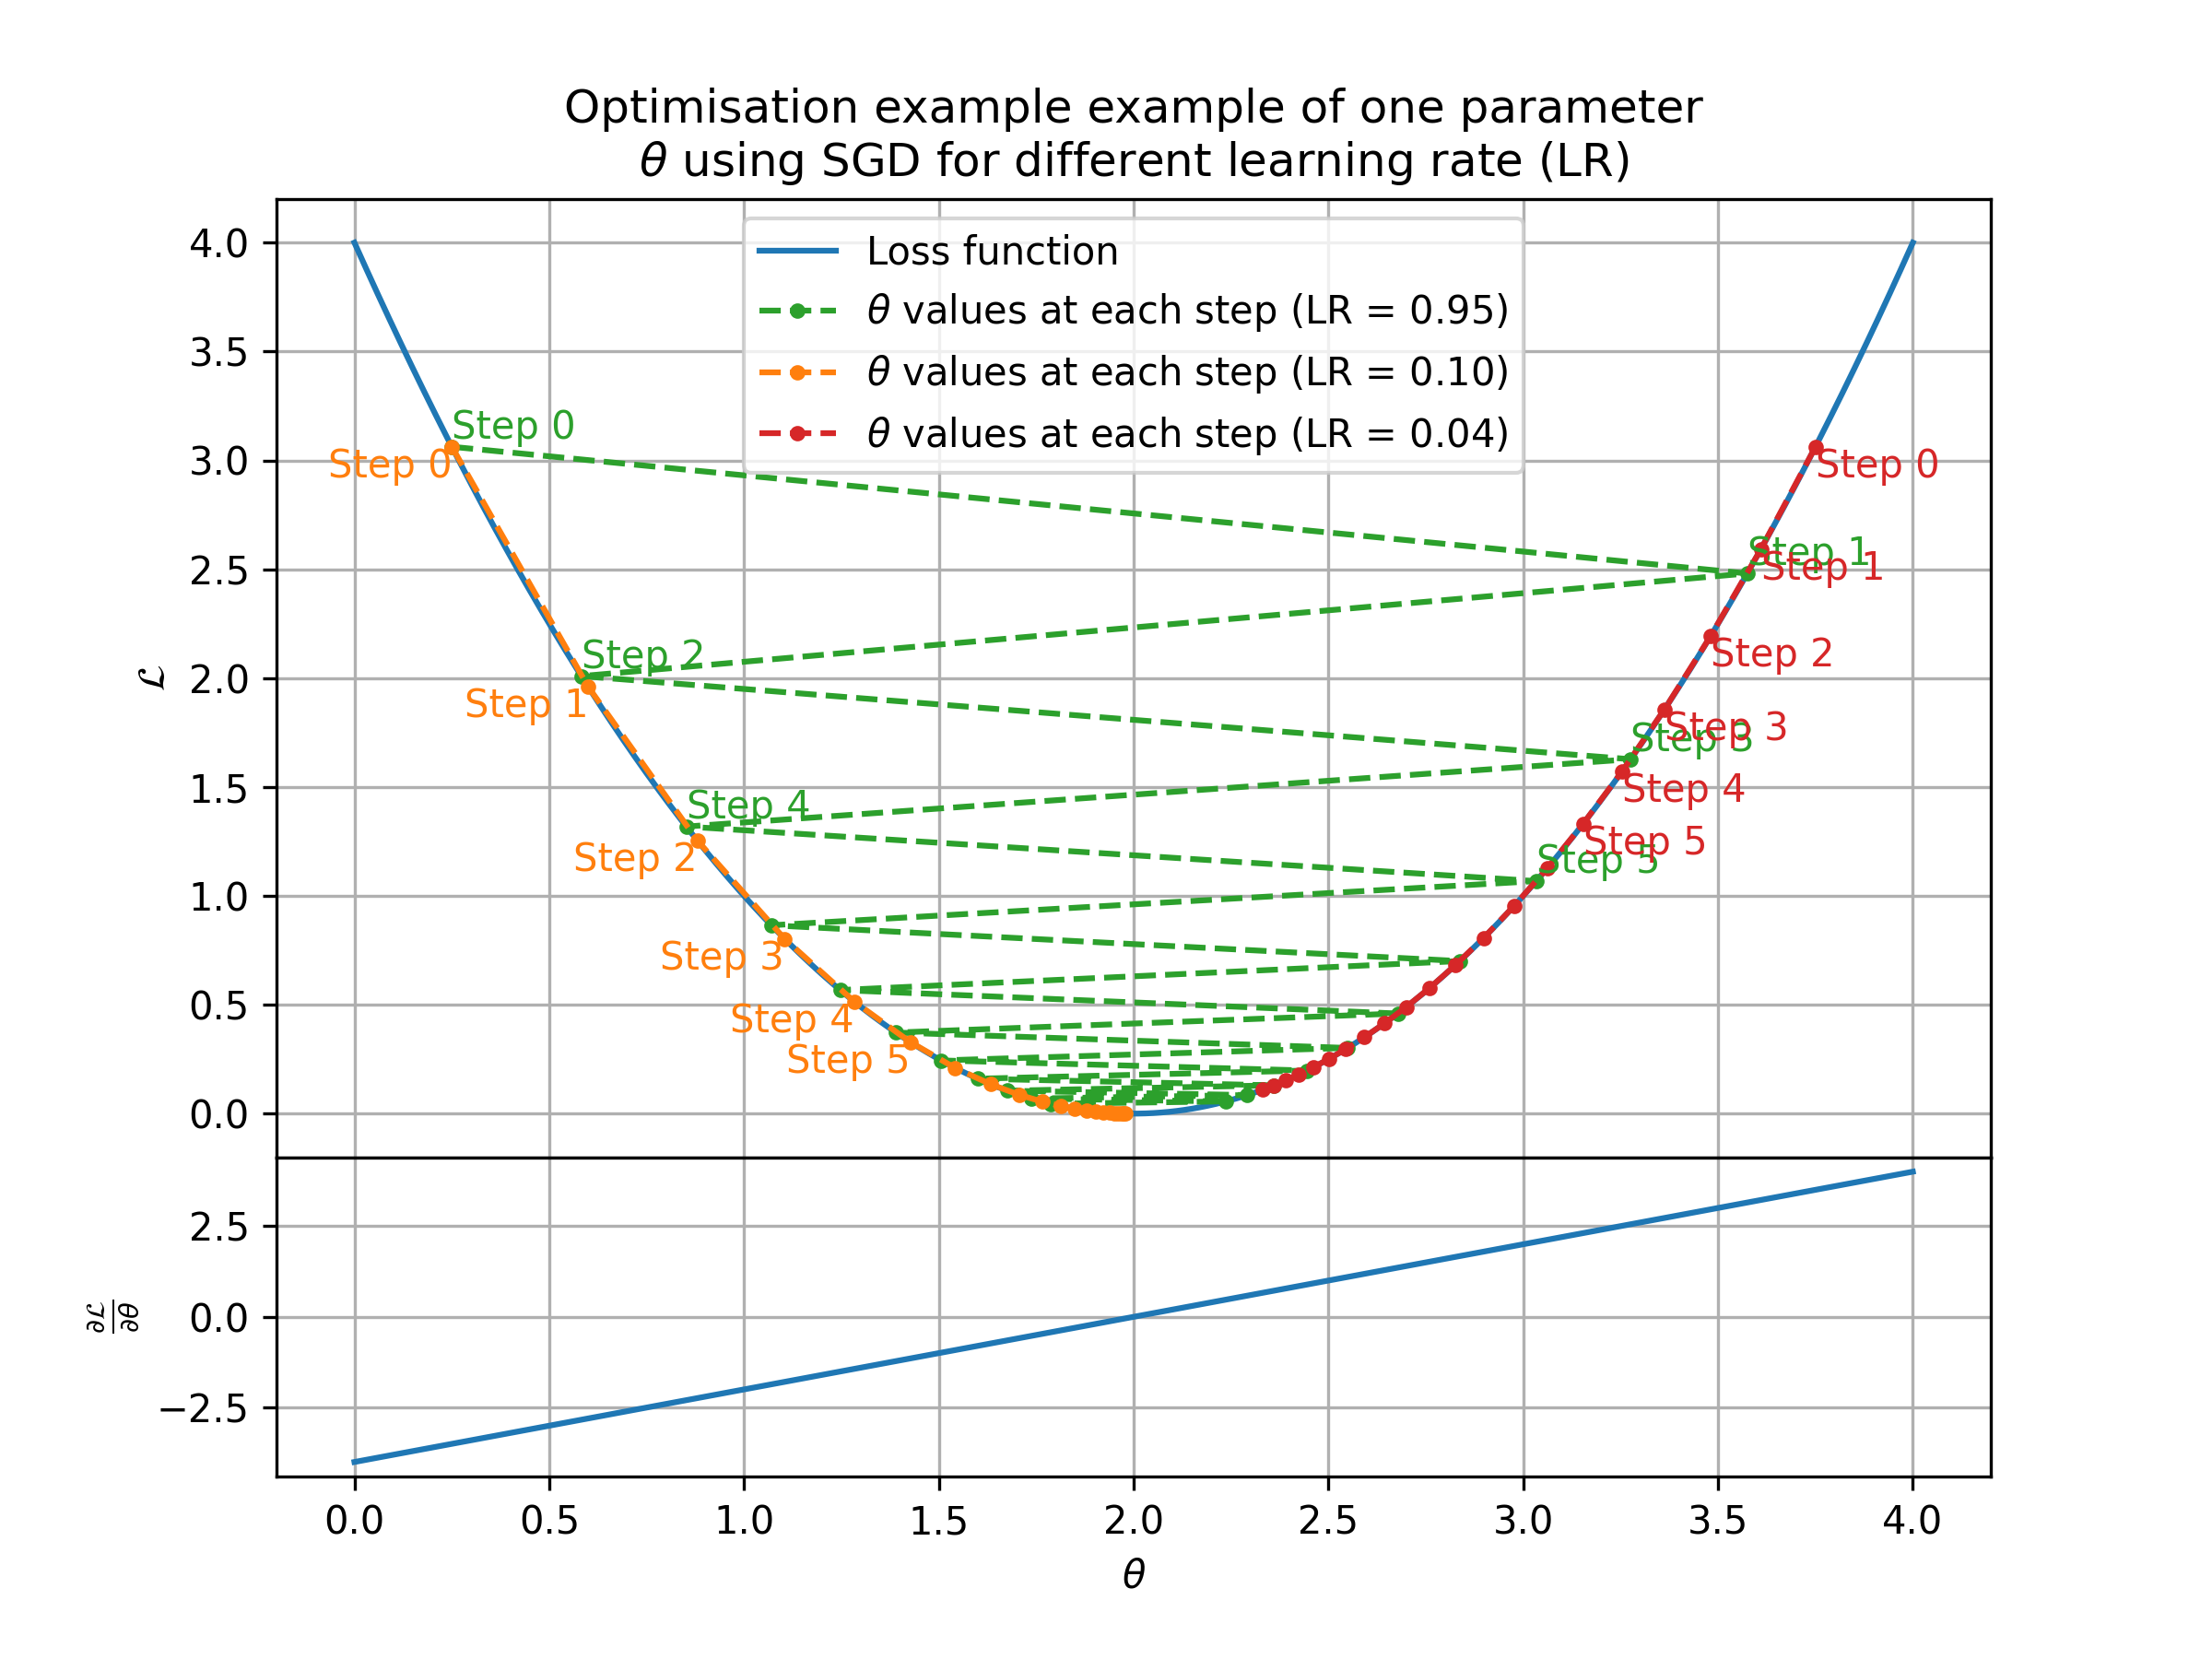
\includegraphics[height=6cm]{scripts/plots/MSE_illustration.png}
    \caption{Illustration of the SGD optimizer on one parameter $\theta$ on the MAE Loss. We see two different behavior: A smooth one (orange and red) when the LR is small enough and a more chaotic one when the LR is too high.}
  \end{subfigure}
  \caption{Illustration of the SGD optimizer. In blue is the value of the loss function, orange, green and red are the path taken by the optimized parameter during the training for different LR.}
  \label{fig:ml:optims}
\end{figure}

\subsubsection{Scheduler policies}

Sometimes we want to update our hyperparameters or take a set of action during the training procedure. We use for this scheduler policies, for example a common policy is a decrease of the learning rate after each epochs. The reasoning is that if the learning rate is too high, the optimizer will continuously miss the minimum and oscillate around it (figure \ref{fig:ml:optims:mae}). By reducing the learning rate, we allow it to make more fine steps in the parameters phase space, hopefully converging to the true minima.

Another policy that is often use is the save of the best model. In some situation, the loss value after each epoch will strongly oscillate or can even worsen. This policy allow us to keep the best version of the model attained during the training phase.

\subsection{Potential pitfalls}
\label{sec:ml:pitfall}

Apart from being stuck in local minima, there is also other behaviors and effects we want to prevent during training.

\subsubsection{Overtraining}
This happen when the network learn the specificities of the training dataset instead of a more general representation of the underlying data distribution. This can happen if there is not enough data in comparison to the number of learning parameters, if the data contains some specific signatures specific to the training dataset or if trains for too long on the same dataset. This behavior is illustrated in figure \ref{fig:ml:overtraining}. Overtraining can be fought in multiple ways, for example:
\begin{itemize}
  \item \textbf{More data}. By having more data in the training dataset, the network will not be able the specificities of every data.
  \item \textbf{Less parameters}. By reducing the number of parameters, we reduce the computing and learning capacities of the network. This will force it to fallback to generalist behaviours.
  \item \textbf{Dropout}. This technique implies to randomly set part of the neural network to 0. By doing this, we force the redundancy in its computing capability and, in a way, modify the data decreasing the possibility for specific learning.
  \item \textbf{Early stopping}. During the training we monitor the network performance over a validation dataset. The network does not train on this dataset and thus cannot learn its specificities. If the loss on the training dataset diverge too much from the loss on the validation dataset, we can stop the training earlier to prevent it from overtraining.
\end{itemize}

\begin{figure}
  \centering
  \begin{subfigure}[t]{0.48\linewidth}
    \centering
    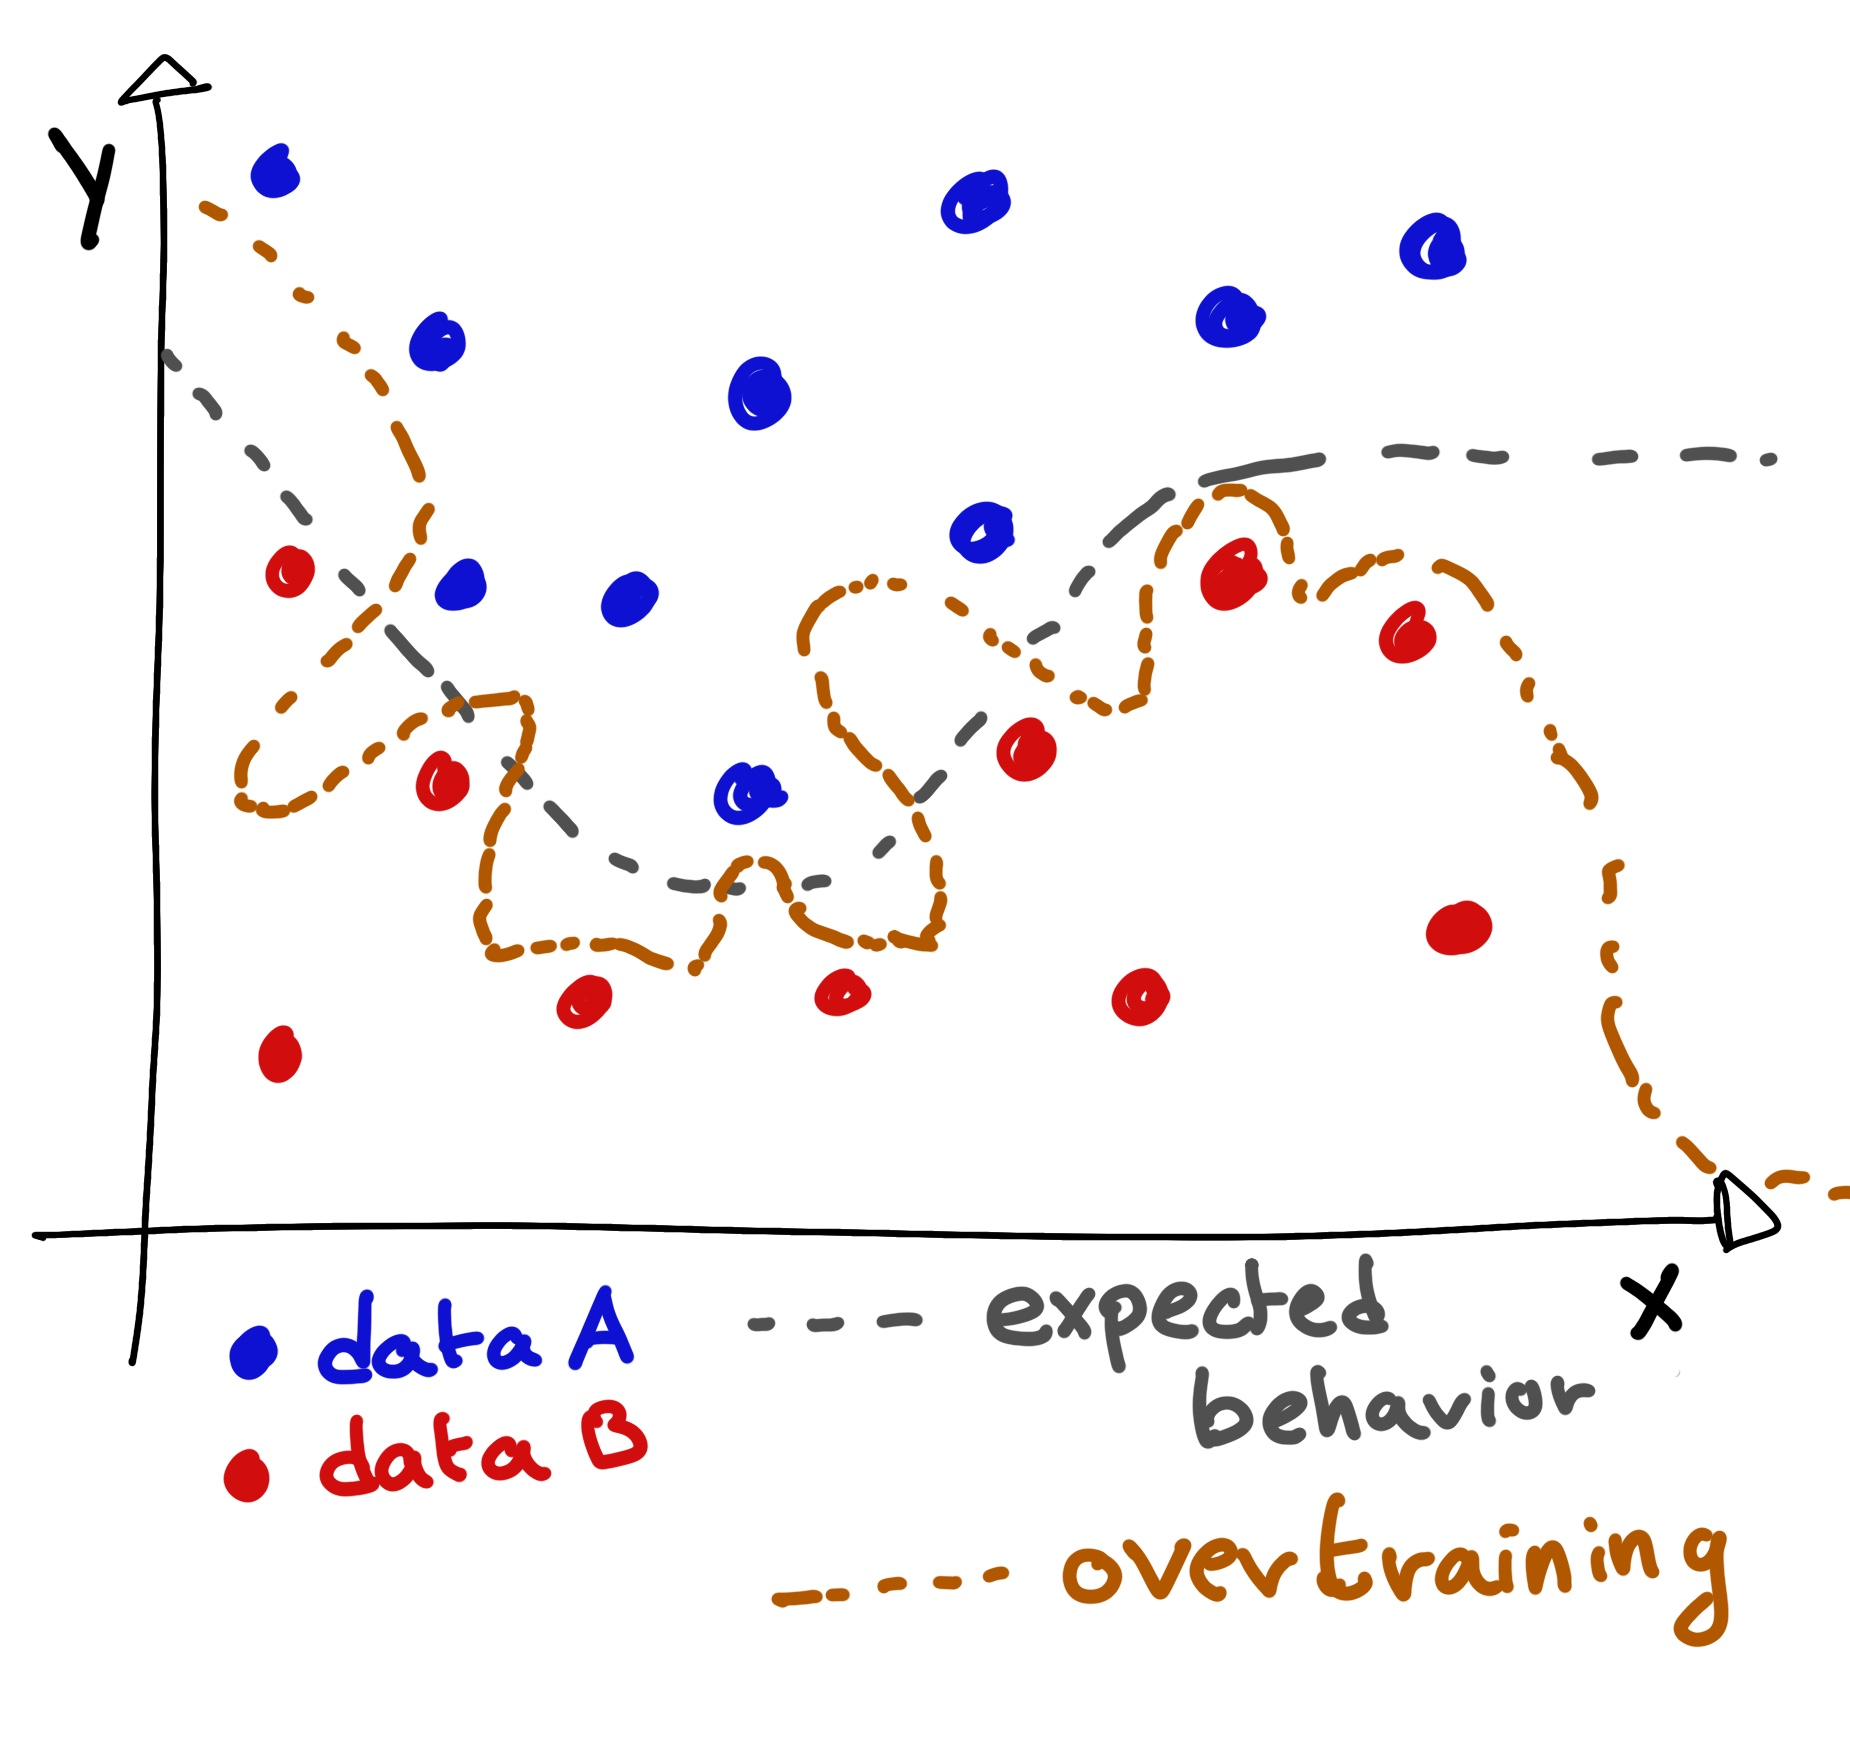
\includegraphics[height=6cm]{images/ml/overtraining.jpg}
    \caption{Illustration of overtraining. The task at hand is to determine depending on two input variable $x$ and $y$ if the data belong to the dataset $A$ or the dataset $B$. The expected boundary between the two dataset is represented in grey. A possible boundary learnt by overtraining is represented in brown.}
    \label{fig:ml:overtraining}
  \end{subfigure}
  \hfill
  \begin{subfigure}[t]{0.48\linewidth}
    \centering
    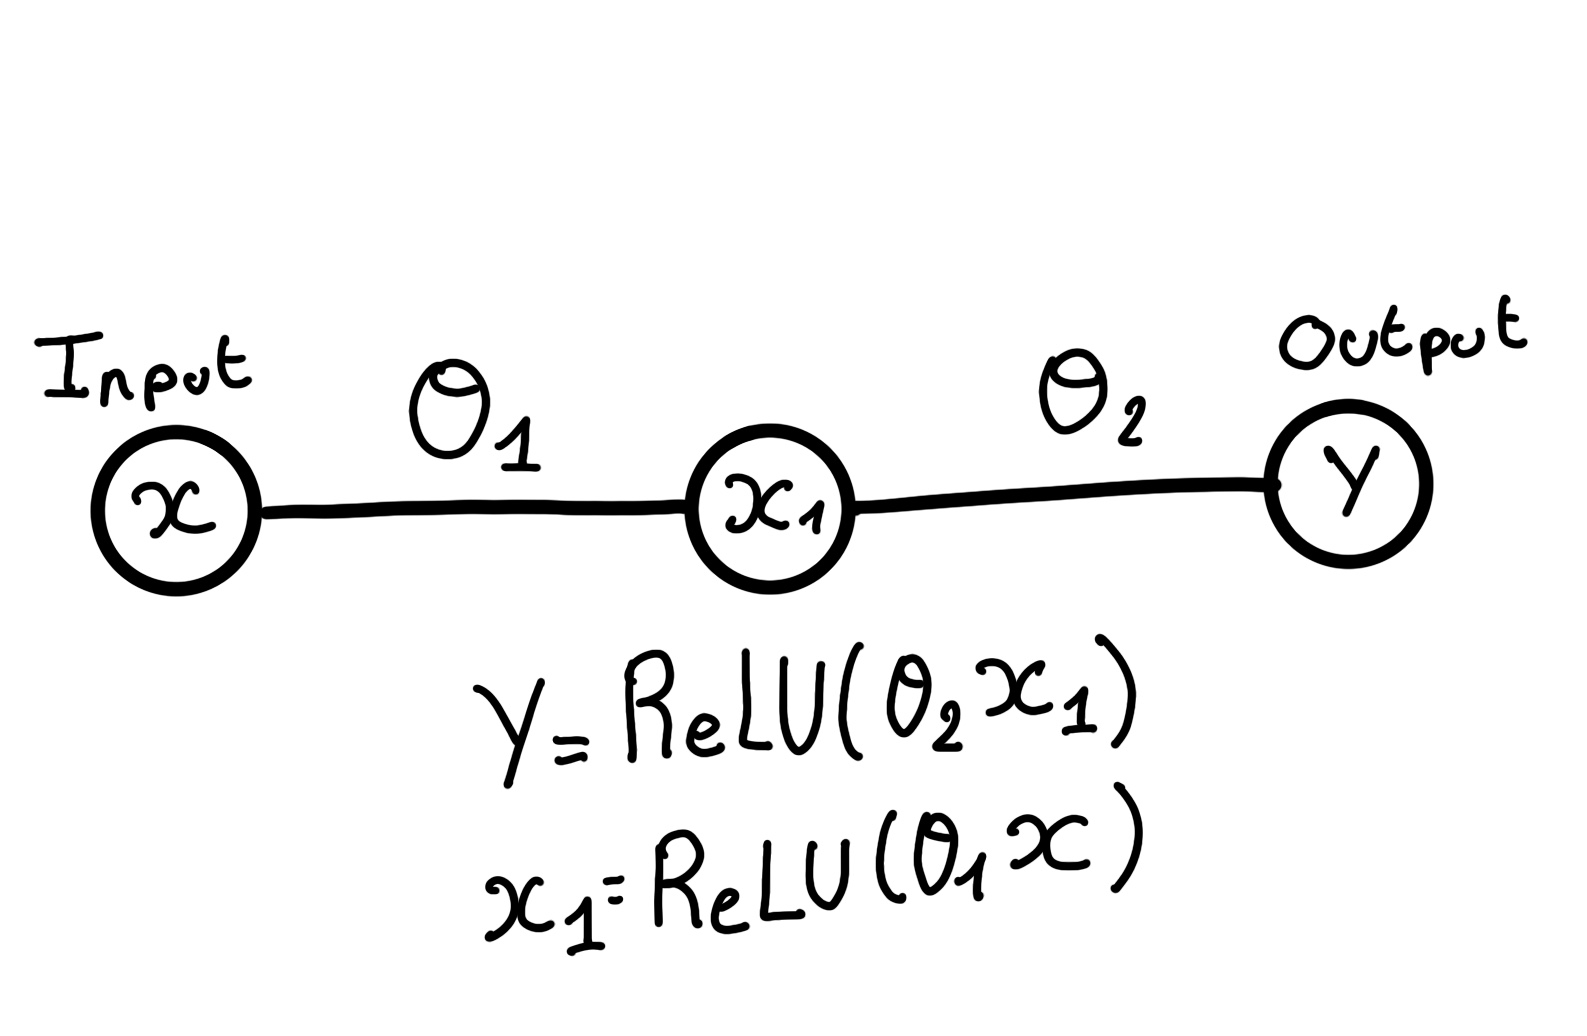
\includegraphics[height=6cm]{images/ml/vanishing_illus.jpg}
    \caption{Illustration of a very simple NN}
    \label{fig:ml:vanishing}
  \end{subfigure}
  \caption{}
\end{figure}

\subsubsection{Gradient vanishing}
Gradient vanishing is the effect of the gradient being so small for the upper layer that the parameters are barely updated after each step. This cause the network to be unable to converge to the minima.

This comes from the way the gradient descent is calculated. Imagine a simple network composed of three fully connected layers: the input layer, a intermediate layer and the output layer. Let $L$ be the loss, $\theta_1$ the parameter between the input and the intermediate layer and $\theta_2$ the parameter between the intermediate and output layer. This network is schematized in figure \ref{fig:ml:vanishing}.

The gradient for $\theta_1$ will be computed using the chain rule presented in equation \ref{eq:ml:backward}. Because $\theta_1$ depends on $\theta_2$, if the gradient of $\theta_2$ is small, so will be the gradient of $\theta_1$. Now if we would have much more layer, we can see how the subsequent multiplication of small gradients would lead to very small update of the parameters thus ``\textit{vanishing gradient}''.

Multiple actions can be taken to prevent this effect such as:
\begin{itemize}
  \item \textbf{Batch normalization}: In this case we apply a normalization layer that will normalize the data so that, let $D$ be the data, $\langle D \rangle = 0$ and $\sigma D = 1$. This help the weight of the network to maintain an appropriate scale.
  \item \textbf{Residual Network (ResNet)} \cite{he_deep_2016}: Residual network is a technique for neural network in which, instead of just sequentially feeding the results of each layer to the next one, you ask each layer to calculate the residual of the input data. This technique is illustrated in figure \ref{fig:ml:resnet}.
\end{itemize}


\begin{figure}[ht]
  \centering
  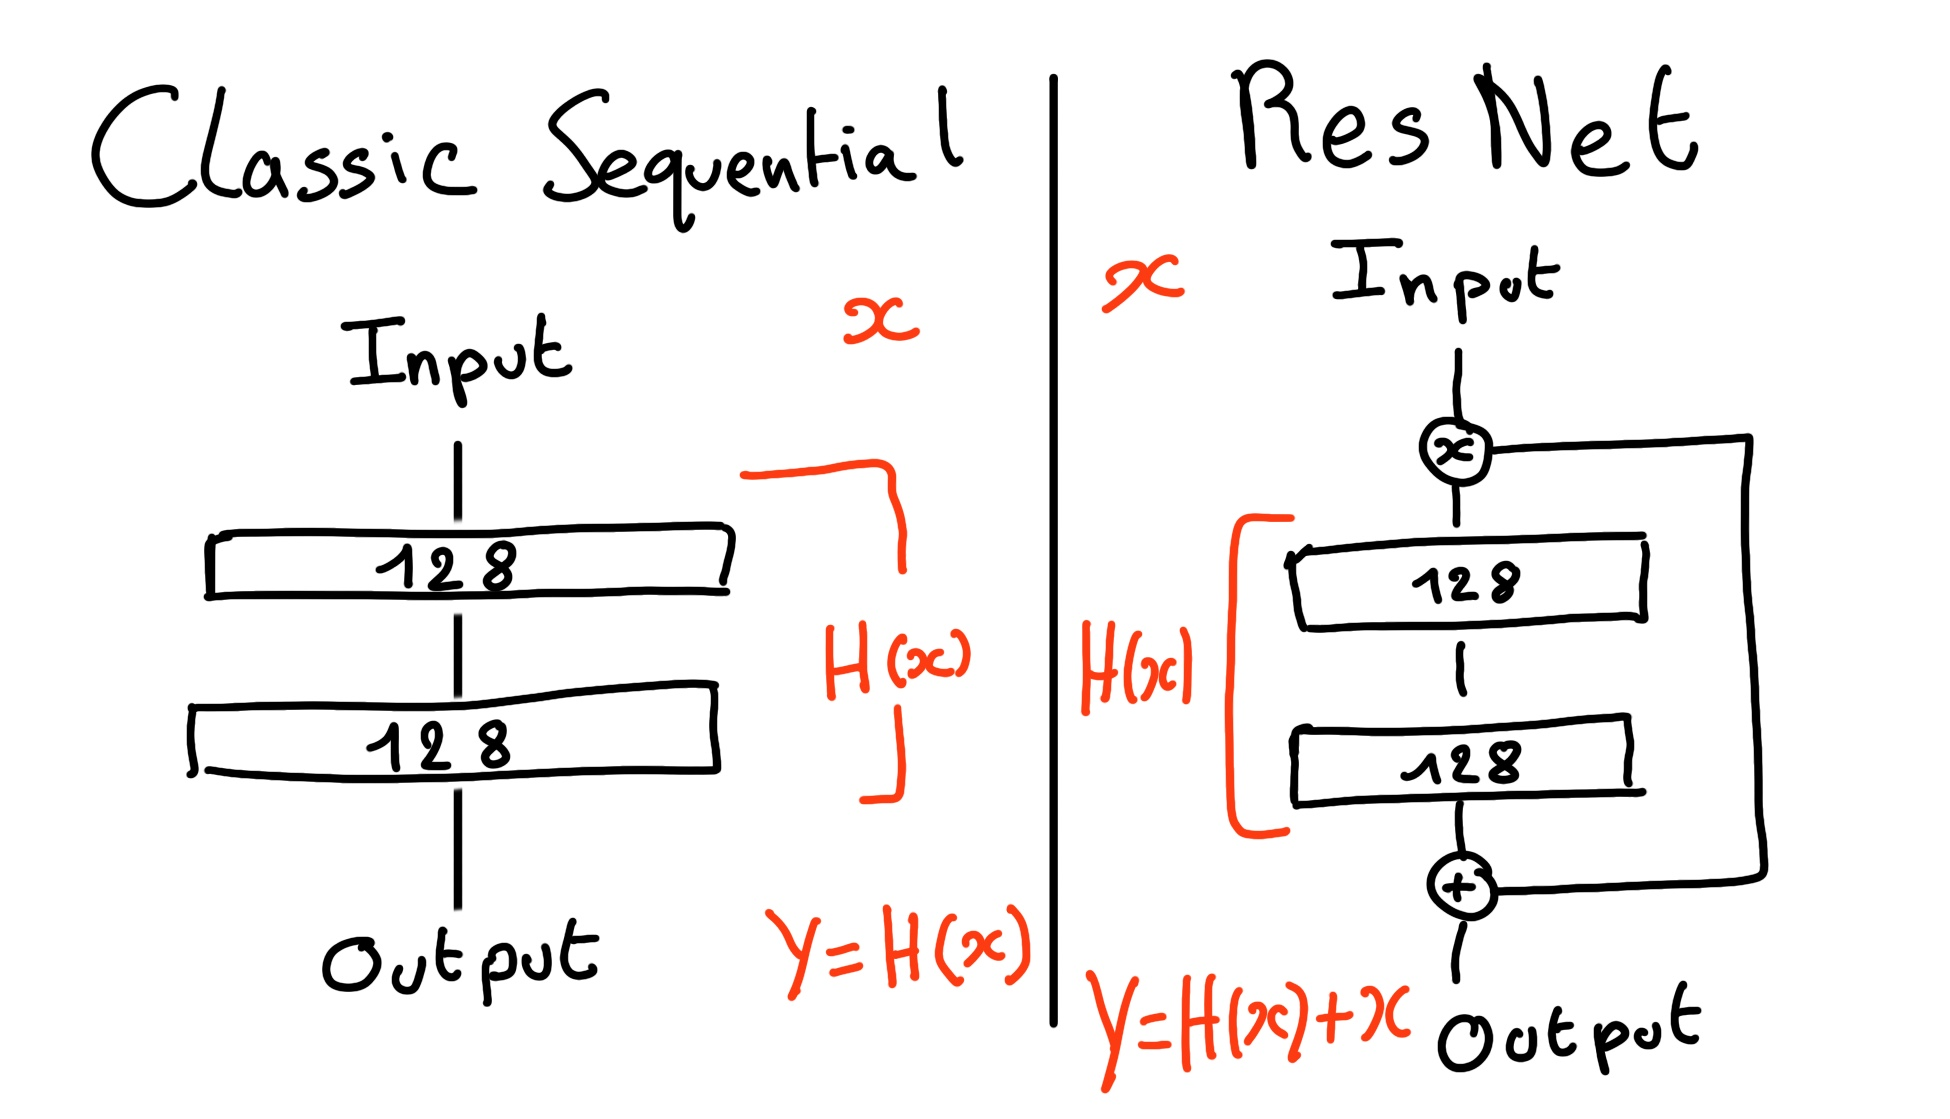
\includegraphics[height=6cm]{images/ml/resnet.jpg}
  \caption{Illustration of the ResNet framework}
  \label{fig:ml:resnet}
\end{figure}

\subsubsection{Gradient explosion}
Gradient explosion happens when the consecutive multiplication of gradient cause exponential grow in the parameter value or if the training lead the network in part of the parameter space where the gradient is significantly higher than usual. For illustration, consider that the loss dependency in $\theta$ follow
\begin{align*}
  \mathcal{L}(\theta) &= \frac{\theta^2}{2} + e^{4\theta} \\
  \frac{\partial \mathcal{L}}{\partial \theta} &= \theta + 4e^{4\theta}
\end{align*}
The explosion is illustrated in figure \ref{fig:ml:explosion} where we can see that the loss degrade with each step of optimization. In this illustration it is clear that reducing the learning rate suffice but this behaviour can happens in the middle of the training where the learning rate schedule does not permit reactivity.

There exist solutions to prevent this explosions:
\begin{itemize}
  \item \textbf{Gradient clipping}: Is this case we work on the gradient so that the norm of gradient vector does not exceed a certain threshold. In our illustration in figure \ref{fig:ml:explosion} the gradient for $\theta > 0$ could be clipped at 3 for example.
  \item \textbf{Batch normalization}: For the same reasons as for gradient vanishing, normalizing the input data help reduce erratic behaviour.
\end{itemize}


\begin{figure}[ht]
  \centering
  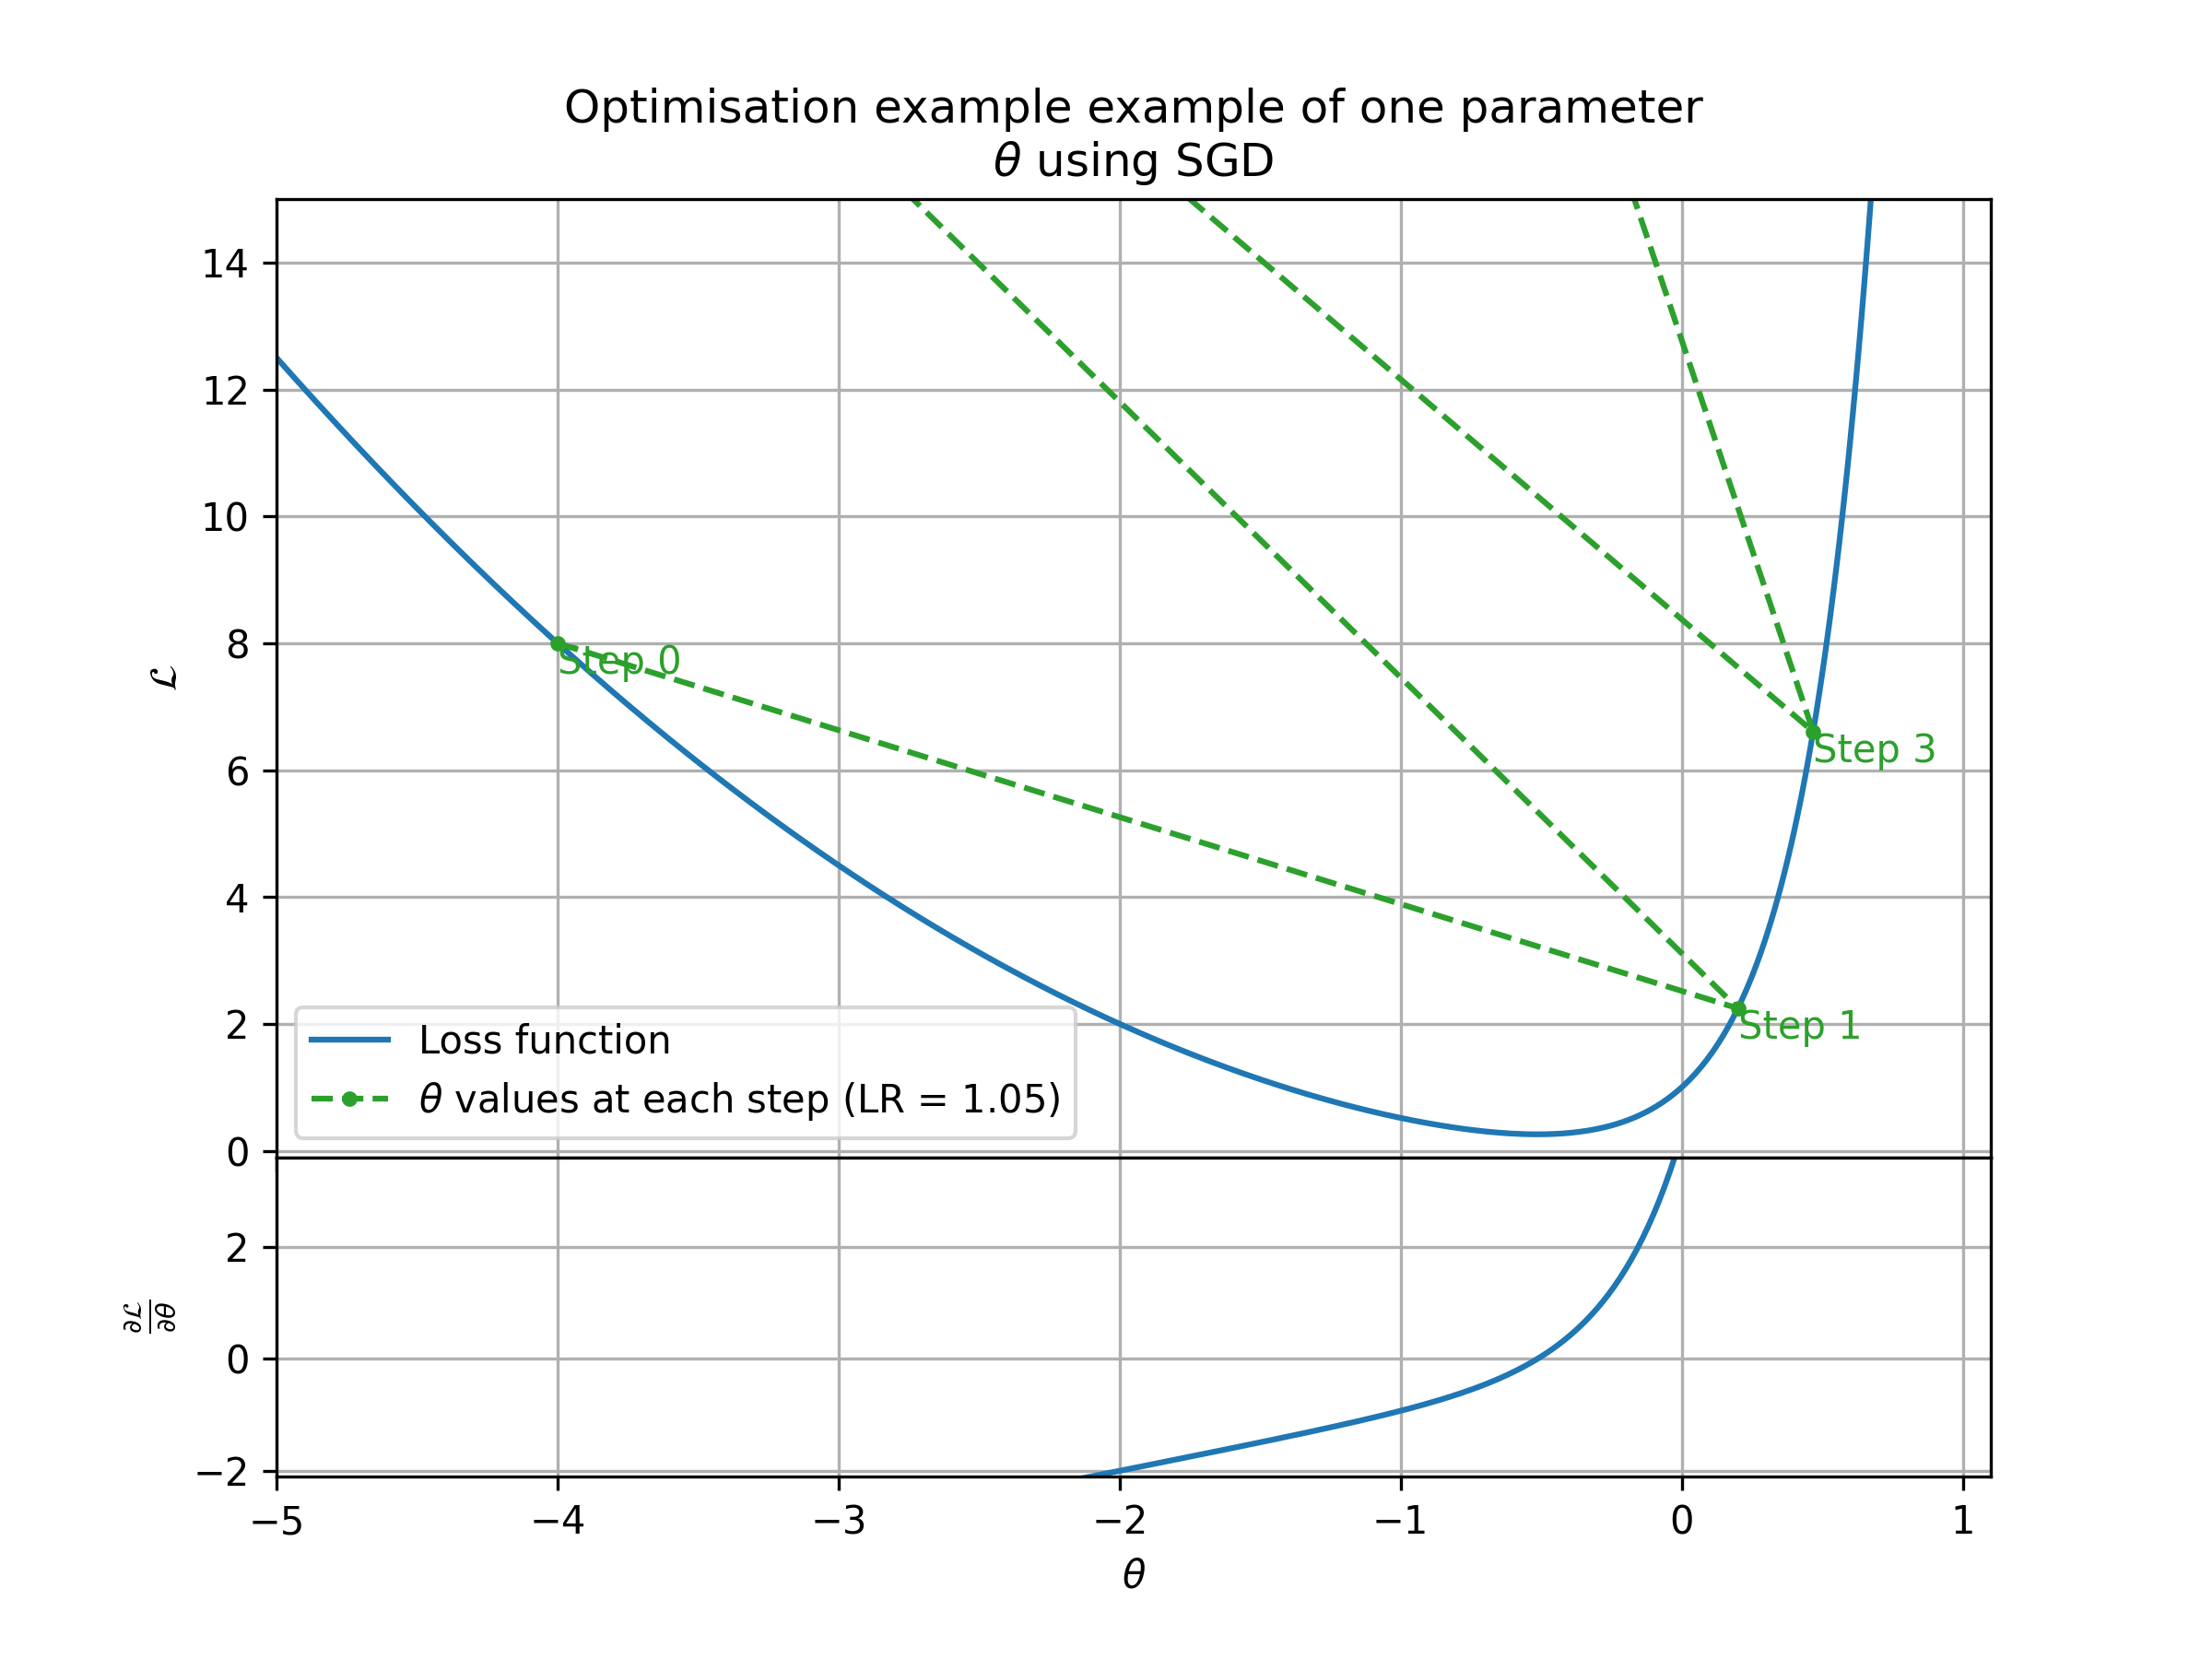
\includegraphics[height=6cm]{scripts/plots/MSE_explosion_illustration.png}
  \caption{Illustration of the gradient explosion. Here it can be solved with a lower learning rate but its not always the case.}
  \label{fig:ml:explosion}
\end{figure}

\end{document}
